\documentclass[a4paper,12pt,titlepage,openany]{bxjsbook}

%%%%%%%%%%%%%%%%%%%%%%%%%%%%%%　スタイルファイル　%%%%%%%%%%%%%%%%%%%%%%%%%%%%%

\usepackage{luatexja}
\usepackage{luatexja-fontspec} % 日本語フォントを扱う（必要なら明示指定）
\usepackage[square, numbers, sort&compress]{natbib}
%本文
\usepackage{ascmac} % 装飾（囲いとか）
\usepackage{enumerate} % 箇条書きのオプション
\usepackage{multicol} %n段組
\usepackage{ulem}
% \usepackage{comment}
%数式
\usepackage{amssymb,amsfonts} % 数学1
\usepackage{mathtools} % 数学2
\usepackage{amsthm} % 数学定理証明環境
\usepackage{mathrsfs} % 花文字
\usepackage{bm} % 太字
\usepackage{cancel} % 取り消し線（相殺）
\usepackage{centernot} % 中央で取り消し線
%\usepackage{physics2} %物理用, ブラケット表示など
\usepackage{braket} 
\usepackage{bbm}
\usepackage{comment} % for \begin{comment}...\end{comment}
% \usepackage{feynmp-auto} % ファインマン（普段使わないならOFF）
% \usepackage[ruled, linesnumbered]{algorithm2e} % アルゴリズム（必要ならON）
\usepackage{caption} % for improved caption handling
\usepackage{fix-cm}
\usepackage{relsize} % 文字サイズ相対変更
\usepackage{physics}
%図表挿入
\usepackage{graphicx} % 画像使うよ
\usepackage{xcolor}
\usepackage{here}
% \usepackage{wrapfig} % 回り込み（必要ならON）
% \usepackage{overpic} % 画像上に描画（必要ならON）
\usepackage{caption}

% 図や表のキャプションを変更
%\captionsetup[figure]{labelformat=default, labelsep=period, name=図~, justification=centering}
%\captionsetup[table]{labelformat=default, labelsep=period, name=表~}

%描画
% \usepackage{tikz} % 図を描く（必要ならON）
\usepackage{tikz}
\usetikzlibrary{shapes.geometric, arrows}
\usepackage{float}
%その他専門性の高いやつ
% \usepackage{fancybox}
% \usepackage{tcolorbox}
% \tcbuselibrary{xparse,hooks,skins,breakable}
% \tcbuselibrary{theorems}
% \usepackage[version=3]{mhchem}

%%%%%%%%%%%%%%%%%%%%%%%%%%%%%%　　　定理環境　　　%%%%%%%%%%%%%%%%%%%%%%%%%%%%%%
%定義, 定理, 証明環境の再定義
% 最小構成にするため一旦OFF（必要になったらON）
% \renewcommand{\proofname}{\doublebox{\textbf{証明}}}
% \newtheorem{dfn}{\textbf{定義}}[subsection]
% \newtheorem{prop}{\textbf{命題}}[subsection]
% \newtheorem{thm}{\textbf{定理}}[subsection]
% \renewcommand{\qedsymbol}{} %証明終了記号を表示しないように変更.

% tcolorbox を使う装飾的な証明環境（必要ならON）
% \DeclareTColorBox{vlinebox}{}{ %縦棒囲い
% enhanced,
% colback=white,
% colframe=white,
% breakable,
% underlay={
% \path[draw, thick, black](frame.north west)--(frame.south west);
% }
% }
% 
% \newcommand{\vlineproof}[1]{
% \begin{proof}
% \begin{vlinebox}
% {\scriptsize
% \setlength{\abovedisplayskip}{0pt}
% \vspace{-6pt}
% #1
% \qed{$\blacksquare$}
% }
% \end{vlinebox}
% \end{proof}
% }

\numberwithin{equation}{section}

%%%%%%%%%%%%%%%%%%%%%%%%%%%%%% フォントなどの設定 %%%%%%%%%%%%%%%%%%%%%%%%%%%%%%

\renewcommand{\thefootnote}{*\arabic{footnote}} % 注釈の設定
\renewcommand{\headfont}{\bfseries} % 章見出しなどのフォント

%%%%%%%%%%%%%%%%%%%%%%%%%%%%%%　しおりとリンク　　%%%%%%%%%%%%%%%%%%%%%%%%%%%%%%
\usepackage[colorlinks=true, linkcolor=blue, citecolor=blue, urlcolor=blue]{hyperref}
\hypersetup{
pdfborder={0 0 0},
breaklinks=true
}

%%%%%%%%%%%%%%%%%%%%%%%%%%%%%%　よく使うコマンドの再定義　　%%%%%%%%%%%%%%%%%%%%%%%%%%%%%%
% 最小限だけ残す（必要になったら追加）
\newcommand{\im}{\mathrm{i}}
\newcommand{\e}{\mathrm{e}}

% \usepackage{colortbl}
% \newcommand\TODO[1]{\textcolor{red}{({\bf TODO}: #1 )}}

%%%%%%%%%%%%%%%%%%%%%%%%%%%%%%　　テンプレート用メタ情報　　%%%%%%%%%%%%%%%%%%%%%%%%%%%%%%
% ここを自分の修論情報に書き換える
%\newcommand{\ThesisYear}{令和X年度修了}
%\newcommand{\ThesisTitleLineA}{修士論文タイトル（1行目）}
%\newcommand{\ThesisTitleLineB}{修士論文タイトル（2行目, 不要なら空にする）}
%\newcommand{\GraduateSchool}{埼玉大学大学院}
%\newcommand{\Department}{理工学研究科 物質科学専攻 物理学PG}
%\newcommand{\StudentID}{XXMSXXX}
%\newcommand{\AuthorName}{氏名}
%\newcommand{\Supervisor}{指導教員 XXXX}

%卒業論文用（必要なら上のブロックを置き換える, or 以下を編集して使う）
 \newcommand{\ThesisYear}{令和7年度卒業}
 \newcommand{\ThesisTitleLineA}{gGAによるMott転移計算}
 \newcommand{\ThesisTitleLineB}{}
 \newcommand{\GraduateSchool}{埼玉大学}
 \newcommand{\Department}{理学部物理学科}
 \newcommand{\StudentID}{22RP026}
 \newcommand{\AuthorName}{東川　喜斗}
 \newcommand{\Supervisor}{指導教員 品岡　寛}

 \newcommand{\ve}{\varepsilon}
\newcommand{\vph}{\varphi}
\newcommand{\si}{\sigma}
\newcommand{\bk}{\bm{k}}
\newcommand{\ua}{\uparrow}
\newcommand{\da}{\downarrow}
\newcommand{\sq}{\sqrt}
\newcommand{\ov}{\frac}
\newcommand{\dgr}{^\dagger}
\newcommand{\h}{\mathcal{H}}
\newcommand{\pr}{^\prime}
\newcommand{\sr}{^*}
\newcommand{\lkaku}{\lbrack}
\newcommand{\rkaku}{\rbrack}
\newcommand{\hV}{\mathcal{V}}
\newcommand{\bE}{\bm{E}}
\newcommand{\hL}{\mathcal{L}}
\newcommand{\br}{\bm{r}}
\newcommand{\hN}{\mathcal{N}}
\newcommand{\hR}{\mathcal{R}}
\newcommand{\hG}{\mathcal{G}}
\newcommand{\hD}{\mathcal{D}}
\newcommand{\hU}{\mathcal{U}}
\newcommand{\hP}{\hat{\mathcal{P}}}
\newcommand{\kako}[1]{ \left( #1 \right)}
\newcommand{\ckako}[1]{ \left \{ #1 \right\}}
\newcommand{\dkako}[1]{ \left[ #1 \right]}
\newcommand{\kakeru}{\times}
\newcommand{\mE}{\mathcal{E}}
\newcommand{\bX}{\bm{X}}
\newcommand{\bramda}{\bm{\lambda}}
\newcommand{\henbi}[2]{\ov{\partial #1}{\partial #2}}
\begin{document}

%%%%%%%%%%%%%%%%%%%%%%%%%%%%%%　　表紙　　%%%%%%%%%%%%%%%%%%%%%%%%%%%%%%
\thispagestyle{empty}
\vspace{7cm}
\begin{center}
{\Large \ThesisYear}

\vspace{5cm}

{\LARGE
\begin{tabular}{c}
\ThesisTitleLineA \\
\ThesisTitleLineB
\end{tabular}}

\vspace{5cm}

{\Large \GraduateSchool}

\vspace{0.1cm}
{\Large \Department}

\vspace{0.1cm}
{\Large 学籍番号　\StudentID}

\vspace{1cm}
{\LARGE \AuthorName}
\vspace{1cm}

{\Large \Supervisor}
\end{center}

\clearpage

%%%%%%%%%%%%%%%%%%%%%%%%%%%%%%　　概要　　%%%%%%%%%%%%%%%%%%%%%%%%%%%%%%
\thispagestyle{empty}
\begin{center}
{\large \textbf{概要}}
\end{center}
\vspace{0.5cm}
\begin{itemize}
    \item \textbf{背景と課題}:
    強相関電子系におけるモット転移を正確に記述する手法として,動的平均場理論が広く用いられている.

    しかしこの理論は,複雑な不純物問題を解くために極めて計算負荷の大きい厳密な数値計算を必要とする課題があった.

    \item \textbf{提案/目的}:
    本研究の目的は,動的平均場理論における無限個の電子の浴を少数のゴースト軌道で置き換える近似手法を用いて,モット転移を定量的かつ極めて低い計算コストで解析することである.

    \item \textbf{手法}:
    最も基礎的な強相関モデルである単一バンドハバードモデルを対象とした.

    物理軌道に加えて2つの空間ゴースト軌道を導入して変分空間を拡張し,自己無撞着な最適化計算を実装した.

    そして,無限次元Bethe格子および2次元正方格子における基底状態の性質を解析した.

    \item \textbf{主結果}:
    相互作用パラメータの増大に伴い,金属相の指標である準粒子重みがゼロとなる金属絶縁体転移を明確に観測した.

    さらに,昇順および降順のスイープ計算を行うことで,一次相転移に特有のヒステリシスループを捉えることに成功した.

    特に無限次元Bethe格子における転移点の臨界値は,動的平均場理論による厳密な計算結果と極めて良い一致を示した.

    \item \textbf{結論/意義}:
    浴の自由度を劇的に削減する大胆な近似を行ったにもかかわらず,本手法はモット転移の物理を高精度に記述できることが証明された.

    厳密対角化を用いて一瞬で解を導出できる圧倒的な計算コストの低さは,本手法が今後より複雑な現実の物質系へ適用可能な強力なツールとなることを示している.
\end{itemize}

\clearpage

%%%%%%%%%%%%%%%%%%%%%%%%%%%%%%　　目次　　%%%%%%%%%%%%%%%%%%%%%%%%%%%%%%
\setcounter{tocdepth}{2}
{
\hypersetup{linkcolor=black}
\tableofcontents
}

\clearpage

%%%%%%%%%%%%%%%%%%%%%%%%%%%%%%　　本編　　%%%%%%%%%%%%%%%%%%%%%%%%%%%%%%
\chapter{序論}
% Chapter 1 placeholder
\section{背景}

物性物理学において,電子間のクーロン相互作用が強く働く強相関電子系の研究は,極めて重要なテーマの一つである.

通常の金属では,電子は互いに独立した自由電子として振る舞うというバンド理論によってその性質がよく記述される.

しかし強相関電子系においては,電子同士の強い斥力によってバンド理論の予測が破綻し,多彩で特異な物理現象が引き起こされる.

その最も代表的な現象が,電子が各原子サイトに局在して金属から絶縁体へと相転移するモット転移である.

このモット転移をはじめとする強相関電子系の振る舞いを記述する最も基礎的な理論模型として,ハバードモデルが広く用いられている.

ハバードモデルは,電子が隣接サイトへ移動する運動エネルギーと,同一サイトに2つの電子が占有した際に生じる局所的なクーロン斥力エネルギーの競合を表現した模型である.

これまで,このハバードモデルにおけるモット転移を解析するための標準的な手法として,動的平均場理論が確立され大きな成功を収めてきた.

動的平均場理論は,格子全体の多体系の問題を,無限個の電子の浴と結合した単一の有効不純物問題にマッピングすることで解を求める強力な手法である.

しかしこの手法は,マッピングされた不純物問題を厳密に解くために,極めて計算負荷の大きい数値計算ソルバーを必要とする.

このような背景から,重い不純物ソルバーを用いずに,極めて低い計算コストでモット転移を定量的に記述できる新しい近似手法の開発が強く求められてきた.

\section{関連研究}

\subsection{動的平均場理論}

強相関電子系の理論的枠組みとして,現在最も成功を収めている手法の一つが動的平均場理論である.

この理論は,空間的な揺らぎを無視する代わりに,時間的な量子揺らぎを厳密に取り扱う手法である.

具体的には,格子上の多体問題を,無限個の自由電子の浴と結合した単一の不純物問題にマッピングして自己無撞着に解を求める.

特に空間次元が無限大の極限においては,この不純物問題へのマッピングが厳密に成立することが知られている.

動的平均場理論は金属状態とモット絶縁体状態の両方を統一的に記述できるため,モット転移の解析における標準的な手法として広く用いられている.

しかし,マッピングされた不純物問題を近似なしに解くためには,連続時間量子モンテカルロ法などの高度な数値計算ソルバーが必要となる.

これらの厳密な不純物ソルバーは極めて計算負荷が大きく,スーパーコンピュータを用いたとしても膨大な計算時間が要求される.

そのため,より複雑な多軌道系や大規模な格子モデルへの適用においては,計算コストの爆発的な増大が研究を進める上での大きな障壁となっている.
\subsection{Gutzwiller近似}
Gutzwiller近似では,クーロン相互作用の効果を取り入れるために次のような相関因子を導入したGutzwiller試行関数を提唱した.
\begin{equation}
    \psi_{\text{G}}=\prod_{j}\dkako{1-\kako{1-g}\hat{n}_{j\ua}\hat{n}_{j\da}}\psi_{\text{0}}=\mathscr{P}_{\text{G}}\psi_{0}.
\end{equation}
ここで\(\psi_{0}\)は自由電子の波動関数であり,ここでは平面波によるフェルミ球を考える.

射影演算子\(\mathscr{P}\)に含まれるパラメータ\(g\)はGutzwiller因子と呼ばれ,\(0<g<1\)である.
つまり電子が二重占有しなければそのまま,二重占有していれば\(g\)倍され,重みが減少する.

この試行関数による変分エネルギーは次で与えられる.
\begin{equation}
\begin{split}
    \ov{E(g)}{N_{s}}&=\ov{\bra{\psi_{\text{G}}}\h\ket{\psi_{\text{G}}}}{N_{s}\braket{\psi_{\text{G}}}}\\
        &=\ov{\bra{\psi_{\text{G}}}-\sum_{i,j,\si}t_{ij}\hat{c}\dgr_{i\si}\hat{c}_{j\si}\ket{\psi_{\text{G}}}+\bra{\psi_{\text{G}}}U\sum_{i}\hat{n}_{i\ua}\hat{n}_{i\da}\ket{\psi_{\text{G}}}}{N_{s}\braket{\psi_{\text{G}}}}.
\end{split}
\label{eq:var_energy}
\end{equation}

\(N_{s}\)はサイト数.

変分法によって\(E(g)\)を\(g\)に対して最小にする.

変分エネルギーの計算をそのままするのは難しいので確率論と近似を用いて求める.

まず全サイト数を\(N_{s}\),各スピンの電子の数を\(N_{\ua}\),\(N_{\da}\),二重占有サイトの数を\(D\)とする.

またサイト数との比として\(n_{\ua}=N_{\ua}/N_{s}\),\(n_{\da}=N_{\da}/N_{s}\),\(d=D/N_{s}\)とする.

\(\psi_{0}\)は各サイトにばら撒かれた電子の状態の重ね合わせである.

この分布が持つ状態を,二重占有サイトの数\(D\)によって分類する.

配置の場合の数を考えると\(N_{s}\),\(N_{\ua}\),\(N_{\da}\)に対して一定の\(D\)を持つ電子配列の数\(N_{D}\)は重複組み合わせを考えて
\begin{equation}
    N_{D}\kako{N_{s},N_{\ua},N_{\da}}=\ov{N_{s}!}{\kako{N_{\ua}-D}!\kako{N_{\da}-D}!D!\kako{N_{s}-N_{\ua}-N_{\da}+D}!}.\label{eq:ND}
\end{equation}

また,サイト占有に対して空間的な相関無視,つまり各サイトに各状態の電子が存在する確率が独立だとすればスピン\(\si\)を持つ\(N_{\si}\)個の電子があるひとつの配列を取る確率は
\begin{equation}
    P\kako{N_{s},N_{\si}}=n_{\si}^{N_{\si}}\kako{1-n_{\si}}^{N_{s}-N_{\si}}.\label{eq:prob}
\end{equation}

このとき波動関数\(\psi_{\text{G}}\)は
\begin{equation}
    \ket{\psi_{\text{G}}}=g^{\hat{D}}\ket{\psi_{0}}
\end{equation}
で表される.

ここで,ある特定の電子配置が指定された状態を\(\ket{\alpha}\)とすれば,規格化因子は完全系で展開して
\begin{equation}
\begin{split}
    \braket{\psi_{\text{G}}}&=\sum_{\alpha}\bra{\psi_{0}}g^{\hat{D}}\ket{\alpha}\bra{\alpha}g^{\hat{D}}\ket{\psi_{\text{0}}}\\
    &=\sum_{\alpha}g^{2D}|\braket{\alpha|\psi_{0}}|^2.
\end{split}
\end{equation}

さらに\(|\braket{\alpha}{\psi_{0}}|^2\)をサイト間の相関を無視し,各サイトにどのスピンの電子が入っているか独立であるとすると,先ほど求めた確率の積で表すことができ

\begin{equation}
    |\braket{\alpha}{\psi_{0}}|^2 \approx P\kako{N_{s},N_{\ua}}P\kako{N_{s},N_{\da}}
\end{equation}
となる.

二重占有数\(D\)になる配置の数は\(N_{D}\kako{N_{s},N_{\ua},N_{\da}}\)であるので
\begin{equation}
    \braket{\psi_{\text{G}}}\approx \sum_{D}g^{2D}N_{D}\kako{N_{s},N_{\ua},N_{\da}}P\kako{N_{s},N_{\ua}}P\kako{N_{s},N_{\da}}
\end{equation}
とかける.

この二重占有サイト数\(D\)に関しての和を解析的に計算するのは容易ではないため熱力学極限\((N_{s}\rightarrow \infty)\)をとり\(D\)に関する和のなかで最大となるものだけを考える.

その項は
\begin{equation}
    \henbi{}{D}\ckako{\ov{g^{2D}}{D!\kako{N_{ua}-D}!\kako{N_{da}-D}!\kako{N_{s}-N_{ua}-N_{da}+D}!}}=0
\end{equation}
という\(D\)が満たす条件をかける\(\kako{このときのDをD^{*}\text{とよぶ}}\).

ここで\(D\)は離散なので,被微分関数を\(F(D)\)とすれば\(F(D^{*}+1),F(D^{*})\)の比が1であればよく
%\begin{equation}
%\begin{split}
 %   &\ov{F(D^{*}+1)}{F(D^{*})}\\
  %  &=\ov{g^{2D^{*}+1}}{g^{2D^{*}}}\ov{D^{*}!}{\kako{D^{*}+1}!}\ov{\kako{N_{\ua}-D^{*}}!}{\kako{N_{ua}-D^{*}-1}!}\ov{\kako{N_{\da}-D^{*}}!}{\kako{N_{\da}-D^{*}-1}!}\ov{\kako{N_{s}-N_{\ua}-N_{\da}+D^{*}}!}{\kako{N_{s}-N{\ua}-N_{\da}+D^{*}+1}!}\\
   % &=g^{2}\ov{1}{D^{*}+1}\kako{N_{\ua}-D^{*}}\kako{N_{\da}-D^{*}}\ov{1}{N_{s}-N_{\ua}-N_{\da}+D^{*}+1}
%\end{split}
%\end{equation}

\begin{small}
\begin{equation}
\begin{split}
    &\ov{F(D^{*}+1)}{F(D^{*})}\\
    &=\ov{g^{2D^{*}+1}}{g^{2D^{*}}}\ov{D^{*}!}{\kako{D^{*}+1}!}\ov{\kako{N_{\ua}-D^{*}}!}{\kako{N_{\ua}-D^{*}-1}!}\ov{\kako{N_{\da}-D^{*}}!}{\kako{N_{\da}-D^{*}-1}!}\ov{\kako{N_{s}-N_{\ua}-N_{\da}+D^{*}}!}{\kako{N_{s}-N_{\ua}-N_{\da}+D^{*}+1}!}\\
    &=g^{2}\ov{1}{D^{*}+1}\kako{N_{\ua}-D^{*}}\kako{N_{\da}-D^{*}}\ov{1}{N_{s}-N_{\ua}-N_{\da}+D^{*}+1},
\end{split}
\end{equation}
\end{small}
と変形できる.

熱力学極限 ($N_s \to \infty$ )の下では,各電子数や二重占有数 $D^*$ もマクロな数となるため,分母の $+1$ は無視して近似できる ($D^* + 1 \simeq D^*$ ).
したがって,比を1とおいた条件式は次のように表される.
\begin{equation}
\begin{split}
    1 &= g^2 \ov{\kako{N_{\ua} - D^*}\kako{N_{\da} - D^*}}{D^* \kako{N_s - N_{\ua} - N_{\da} + D^*}} \\[1ex]
    g^2 &= \ov{D^* \kako{N_s - N_{\ua} - N_{\da} + D^*}}{\kako{N_{\ua} - D^*}\kako{N_{\da} - D^*}}.
\end{split}
\label{eq-g^2}
\end{equation}

最後に,各変数を全サイト数 $N_s$ で割ってサイトあたりの密度 ($d^* = D^*/N_s$,$n_{\ua} = N_{\ua}/N_s$,$n_{\da} = N_{\da}/N_s$ )で書き換える.
右辺の分母と分子をそれぞれ $N_s^2$ で割ることで
\begin{equation}
    g^2 = \ov{d^* \kako{1 - n_{\ua} - n_{\da} + d^*}}{\kako{n_{\ua} - d^*}\kako{n_{\da} - d^*}}.
\end{equation}

同様の計算法を式(\ref{eq:var_energy})の分子にも適用する. まず, $\langle \Psi_G | \sum_{i,j} t_{ij} c_{i\uparrow}^\dagger c_{j\uparrow} | \Psi_G \rangle$ の運動エネルギー項を考える. 
スピン $\uparrow$ を持つ電子が $j$ サイトから $i$ サイトへ跳び移る場合, ホッピング後の状態には必ず $i$ サイトに $\uparrow$ スピンが存在し, ホッピング前の状態には必ず $j$ サイトに $\uparrow$ スピンが存在する. この性質を用いると, サイト $i, j$ における Gutzwiller 因子は $n_{i\uparrow}=1, n_{j\uparrow}=1$ と置き換えることができ, 以下の形に変形できる
\begin{equation}
    \langle \Psi_G | c_{i\uparrow}^\dagger c_{j\uparrow} | \Psi_G \rangle = 
    \langle \Phi_F | c_{i\uparrow}^\dagger c_{j\uparrow} (\bar{n}_{i\downarrow} + g n_{i\downarrow})(\bar{n}_{j\downarrow} + g n_{j\downarrow})\prod_{l \neq i,j} [1 - (1-g)n_{l\uparrow}n_{l\downarrow}]^2 | \Phi_F \rangle .
    \label{eq:hopping_Gutzwiller}
\end{equation}
ここで, $\bar{n}_{i\sigma} = 1 - n_{i\sigma} = c_{i\sigma} c_{i\sigma}^\dagger$ は空サイトを示す演算子である. 
式(\ref{eq:hopping_Gutzwiller})のカッコを展開すると, 4つの項が生じる. 
二重占有数 $D$ が変化しない跳び移りが2つ, 跳び移りの前後で $D$ の数が増減する過程が2つである. 本来 $U \neq 0$ であればこれらは異なる確率で生じるが, GAではこうした局所配置依存性を無視し, 独立な確率の積で置き換える近似を行う. 

各過程について, $i, j$ の2サイトを除外した残り $N_s - 2$ サイト上にある電子配列の組み合わせを数え上げる. このとき, 1つの $\uparrow$ スピンが跳び移るために配置が固定されるため, 残りの $\uparrow$ 電子数は $N_\uparrow - 1$ となる. 
以上の近似と組み合わせの数 (式\ref{eq:ND} )および確率 (式\ref{eq:prob} ))を用いることで, 運動エネルギーの期待値は次のように求まる.
\begin{equation}
\begin{split}
    \langle \Psi_G | \sum_{i,j} t_{ij} c_{i\uparrow}^\dagger c_{j\uparrow} | \Psi_G \rangle 
    &\simeq \sum_D g^{2D} \Big[ N_D(N_s-2, N_\uparrow-1, N_\downarrow)+ g^2 N_D(N_s-2, N_\uparrow-1, N_\downarrow-2)\\
    &\qquad\qquad + 2g N_D(N_s-2, N_\uparrow-1, N_\downarrow-1)\Big] \\
    &\quad \times P(N_s-2, N_\uparrow-1)P(N_s, N_\downarrow)\bar{\epsilon}_\uparrow .
\end{split}
\label{eq:kin_energy_expectation}
\end{equation}

ここで
\begin{equation}
    \bar{\epsilon}_\sigma \equiv - \sum_{i,j} \frac{t_{ij}}{N_s} \langle \Phi_F | c_{i\sigma}^\dagger c_{j\sigma} | \Phi_F \rangle 
    \label{eq:free_energy}
\end{equation}
としている.

また, 式(\ref{eq:var_energy})の同一サイト斥力 (相互作用 )相関の項についても同様に計算を行う. $n_{i\uparrow}n_{i\downarrow}$ が作用するサイト $i$ は確実に二重占有となるため, 因子から $g^2$ が生じ, 残り $N_s - 1$ サイトの組み合わせを考えればよい
\begin{equation}
\begin{split}
    \langle \Psi_G | U \sum_i n_{i\uparrow} n_{i\downarrow} | \Psi_G \rangle 
    &= U g^2 \sum_i \langle \Phi_F | n_{i\uparrow} n_{i\downarrow} \prod_{l \neq i} [1 - (1-g)n_{l\uparrow}n_{l\downarrow}]^2 | \Phi_F \rangle \\
    \simeq N_s U \sum_D g^{2D+2} N_D&(N_s-1, N_\uparrow-1, N_\downarrow-1)P(N_s, N_\uparrow)P(N_s, N_\downarrow).
\end{split}
\label{eq:int_energy_expectation}
\end{equation}

式(\ref{eq:kin_energy_expectation})と式(\ref{eq:int_energy_expectation})を, 規格化因子 (全確率 )である式(1.13)で割ることで, 各エネルギーの期待値が得られる. 

ここでは熱力学極限の下で, 和の中で最大となる $D^*$ の項のみを評価する. 
相互作用エネルギーの期待値は, 組み合わせの数の比をとり $d^* = D^*/N_s$ を用いると, 次のように求まる.
\begin{equation}
    \frac{\langle \Psi_G | U \sum_i n_{i\uparrow} n_{i\downarrow} | \Psi_G \rangle}{N_s \langle \Psi_G | \Psi_G \rangle} 
    \simeq U \frac{g^{2D^*+2} N_{D^*}(N_s-1, N_\uparrow-1, N_\downarrow-1)}{g^{2D^*} N_{D^*}(N_s, N_\uparrow, N_\downarrow)} 
    = U d^* .
    \label{eq:int_energy_final}
\end{equation}

一方, 運動エネルギーの期待値についても同様に比を計算し, 式\ref{eq-g^2}用いて変数 $g$ を消去すると, 次の形に整理される
\begin{equation}
    \frac{\langle \Psi_G | \sum_{i,j} t_{ij} c_{i\uparrow}^\dagger c_{j\uparrow} | \Psi_G \rangle}{N_s \langle \Psi_G | \Psi_G \rangle} 
    \simeq \frac{\left[ \sqrt{(n_\uparrow - d^*)(1 - n_\uparrow - n_\downarrow + d^*)} + \sqrt{(n_\downarrow - d^*)d^*} \right]^2}{n_\uparrow(1 - n_\uparrow)} \bar{\epsilon}_\uparrow .
    \label{eq:kin_energy_final}
\end{equation}
ここで, $\bar{\epsilon}_\sigma$ は式(\ref{eq:free_energy})で定義した非相関時の自由電子の平均運動エネルギーである.

以降, $d^*$ を単に $d$ と表記する. 
式(\ref{eq:kin_energy_final})の係数部分は, 電子相関によってホッピング項を減少させる「準粒子繰り込み因子」$\gamma_\sigma$ として定義される.
\begin{equation}
    \gamma_\sigma = \frac{\left[ \sqrt{(n_\sigma - d)(1 - n_\sigma - n_{-\sigma} + d)} + \sqrt{(n_{-\sigma} - d)d} \right]^2}{n_\sigma(1 - n_\sigma)} \le 1 .
    \label{eq:gamma_factor}
\end{equation}
これらを用いると, GAによるサイトあたりの変分エネルギー $E_{GA} / N_s$ は次のようにシンプルな形で記述できる.
\begin{equation}
    \frac{E_{GA}}{N_s} = \sum_\sigma \gamma_\sigma \bar{\epsilon}_\sigma + U d .
    \label{eq:E_GA}
\end{equation}

\subsubsection{Brinkman-Rice 転移}
Brinkman と Rice は, この GA の結果をハーフフィリング ($n_\uparrow = n_\downarrow = 1/2$, すなわち $n = 1$ )の場合に適用し, モット絶縁体への転移 (Brinkman-Rice 転移 )を見事に記述した. 
$n_\sigma = 1/2$ を式(\ref{eq:gamma_factor})および式\ref{eq-g^2}に代入すると, 因子 $\gamma$ と変分パラメータ $g$ は $d$ のみの関数として次のように求まる.
\begin{equation}
    \gamma \equiv \gamma_\uparrow = \gamma_\downarrow = \frac{\left[ \sqrt{(1/2 - d)d} + \sqrt{(1/2 - d)d} \right]^2}{1/4} = 8d(1 - 2d)
    \label{eq:gamma_half}
\end{equation}
\begin{equation}
    g^2 = \frac{d \cdot d}{(1/2 - d)^2} \quad \Rightarrow \quad g = \frac{2d}{1 - 2d} .
    \label{eq:g_half}
\end{equation}
ここで, 自由電子の運動エネルギーの和を $\sum_\sigma \bar{\epsilon}_\sigma = -|\bar{\epsilon}_0|$ とおくと, 式(\ref{eq:E_GA})の全エネルギーは以下のようになる.
\begin{equation}
    \frac{E_{GA}}{N_s} = -8d(1 - 2d)|\bar{\epsilon}_0| + Ud .
    \label{eq:E_GA_half}
\end{equation}
基底状態のエネルギーを求めるため, これを $d$ について微分し, $\partial (E_{GA}/N_s)/ \partial d = 0$ を課して最適化を行う.
\begin{equation}
    -8|\bar{\epsilon}_0| + 32d|\bar{\epsilon}_0| + U = 0 \quad \Rightarrow \quad d = \frac{1}{4} \left( 1 - \frac{U}{8|\bar{\epsilon}_0|} \right).
    \label{eq:d_optimization}
\end{equation}
この式から, クーロン斥力 $U$ がある臨界値 $U_c^{BR} \equiv 8|\bar{\epsilon}_0|$ に達すると, 二重占有密度が $d = 0$ となり, 電子が各サイトに完全に局在するモット絶縁体状態が実現することがわかる. この $U_c^{BR}$ を用いて $d$, $\gamma$, および最小化されたエネルギー $E_{GA}/N_s$ を書き直すと, 以下のようになる.
\begin{equation}
    d = \frac{1}{4} \left( 1 - \frac{U}{U_c^{BR}} \right)
    \label{eq:d_final}
\end{equation}
\begin{equation}
    \gamma = 1 - \left( \frac{U}{U_c^{BR}} \right)^2 
    \label{eq:gamma_final}
\end{equation}
\begin{equation}
    \frac{E_{GA}}{N_s} = -|\bar{\epsilon}_0| \left[ 1 - \frac{U}{U_c^{BR}} \right]^2 .
    \label{eq:E_GA_final}
\end{equation}
このように, GAを用いることで, 相互作用の増大に伴いホッピングの確率が減少し ($\gamma \to 0$ ), 最終的に金属から絶縁体への相転移が起きる様子が解析的に示された.

\section{本研究の目的}

強相関電子系の理論的研究において, 動的平均場理論 (DMFT)は無限次元極限で厳密となる強力な手法であり, モット絶縁体転移などの複雑な物理現象の解明に多大な貢献をしてきた. 

しかし, DMFTは有効不純物問題の求解 (不純物ソルバー )にかかる計算コストが非常に高く, 複雑な多軌道系や大規模な格子系への適用には実用上の限界が存在する. 

一方, 前節までで定式化を追った Gutzwiller近似 (GA)アプローチは, 計算コストが圧倒的に低いという強力な利点を持つ. 

しかし従来のGAは, 参照する単一粒子波動関数を物理的なヒルベルト空間内に直接構築し, その内部だけで局所的な重みを調整するため, 変分空間の表現力に制限があり, 精度面での妥協を余儀なくされていた. 

そこでDMFTよりも計算コストが軽く, かつGAよりも精度の高い次世代の計算手法として, ghost Gutzwiller近似 (gGA)に着目する.

gGAの最大の特長は, 従来のGAの枠組みに「ゴースト (ghost )」と呼ばれる補助的なフェルミオン自由度を導入する点にある. 

ゴースト自由度を含む仮想的な補助ヒルベルト空間 (Auxiliary space )に参照状態を構築し, そこから現実の物理空間へのマッピングを行うことで, 変分空間を体系的かつ柔軟に拡張する. 

この拡張により, gGAはGAの簡便な計算アルゴリズムを維持したまま, DMFTに匹敵する高精度な相関効果の記述が可能となることが示唆されている. 

本論文の目的は, このgGAの理論的枠組みをハバードモデルに適用し, 従来のGAやDMFTの結果と比較することで, gGAがモット転移をどのように記述するかを明らかにすることである.
\section{本論文の構成}

本論文の構成は以下の通りである.

第1章では,本研究の背景と関連研究について概観し,本研究の目的を述べる.

第2章では,本研究の理論的基礎となるハバードモデルやGutzwiller近似の定式化について解説する.

第3章では,数値計算の対象となる格子モデルやパラメータなどの問題設定について記述する.

第4章では,ghost Gutzwiller近似を用いた具体的な最適化アルゴリズムと計算条件について説明する.

第5章では,無限次元Bethe格子および2次元正方格子における計算結果を示し,動的平均場理論の厳密解との比較を通して考察を行う.

第6章では,本研究で得られた知見を総括し,今後の展望についてまとめる.



\chapter{基礎理論}
% Chapter 2 placeholder

本章では, 本研究で対象とする物理系を記述する理論モデルと, その解析に用いる計算手法について述べる. まず基本となるハバードモデルについて概説し,本研究の主眼である ghost Gutzwiller 近似 (gGA)の定式化について詳細を解説する. 

\section{ハバードモデル}

強相関電子系の理論的研究において, ハバードモデル (Hubbard model)は電子間の局所的なクーロン相互作用と非局所的な運動エネルギーの競合を記述する, 最も基礎的かつ重要な模型である. 
本研究で扱う多軌道系も含む一般的なハバードモデルのハミルトニアン $\hat{H}$ は, 局所的な相互作用項と非局所的なホッピング (跳び移り)項の和として, 以下のように定式化される.
\begin{equation}
    \hat{H} = \sum_{i=1}^{\mathcal{N}} \hat{H}_{loc}^i[c_{i\alpha}^\dagger, c_{i\alpha}] + \sum_{i \neq j} \hat{T}_{ij}.
    \label{eq:hubbard_general}
\end{equation}
\begin{equation}
    \hat{T}_{ij} = \sum_{\alpha=1}^{\nu_i} \sum_{\beta=1}^{\nu_j} [t_{ij}]_{\alpha\beta} c_{i\alpha}^\dagger c_{j\beta}.
    \label{eq:hopping_general}
\end{equation}
ここで, $i$ および $j$ は格子を構成するサイトのインデックスを表し, $\mathcal{N}$ は全サイト数である. 

$\alpha$ および $\beta$ は各サイト内のフェルミオンモード (軌道やスピン自由度)のインデックスであり, $\nu_i$ はサイト $i$ におけるモード数を表す. 
第1項の $\hat{H}_{loc}^i$ はサイト $i$ における任意の局所演算子であり, 1体項や電子間の強いクーロン斥力を表す2体相互作用項を含む. 

第2項の $\hat{T}_{ij}$ は異なるサイト $i, j$ 間の電子のホッピングを表し, $[t_{ij}]_{\alpha\beta}$ はその遷移確率を与える行列要素である. 

前章で議論した Gutzwiller 近似の基礎となる単一バンドモデル (各サイトに軌道が1つでスピン $\sigma = \uparrow, \downarrow$ のみを持つ場合)においては, 式(\ref{eq:hubbard_general})は以下のような馴染み深い形に簡略化される.
\begin{equation}
    \hat{H} = -t \sum_{\langle i,j \rangle, \sigma} \left( c_{i\sigma}^\dagger c_{j\sigma} + H.c. \right)+ U \sum_i n_{i\uparrow} n_{i\downarrow}.
    \label{eq:hubbard_single}
\end{equation}
ここで, 第1項の $t$ は最隣接サイト $\langle i,j \rangle$ 間のホッピング積分, 第2項の $U$ は同一サイトに2つの電子が占有した (二重占有)際に生じるクーロン斥力エネルギーである. 
このモデルは外見こそ単純であるものの, $U$ と $t$ の比 ($U/t$)によって, 電子が自由に動き回る金属状態から, 強い斥力によって電子が各サイトに局在するモット絶縁体状態への転移 (モット転移)など, 豊かな物理現象を記述することができる. 

以降の節では, このハバードモデルを解くための近似手法であるgGAについて定式化を行う.
\section{定義}
\subsection{Gutzwiller変分関数}
Gutzwiller変分関数を次の形で導入する.
\begin{equation}
\Ket{\Psi_{\text{G}}}=\hat{\mathcal{P}}_{\text{G}}\Ket{\Psi_{0}},\quad\hP_{\text{G}}=\prod_{i=1}^{\mathcal{N}}\hP_{i}.
\end{equation}
ここで\(\Ket{\Psi_{0}}\)は補助空間の1粒子状態波動関数であり,\(\Ket{\Psi_{\text{G}}}\)は物理空間の波動関数である.
\begin{align}
    \hP_{i}&=\sum_{\Gamma=0}^{2^{\nu_{i}}-1}\sum_{n=0}^{2^{B\nu_{i}}-1}\dkako{\Lambda_{i}}_{\Gamma{n}}\Ket{\Gamma,i}\Bra{n,i}\\
    \Ket{\Gamma,i}&=\dkako{c\dgr_{i1}}^{q_{1}(\Gamma)}\cdots \dkako{c\dgr_{i\nu_{i}}}^{q_{\nu_{i}}(\Gamma)}\Ket{0}\\
    \Ket{n,i}&=\dkako{f\dgr_{i1}}^{q_{1}(n)}\cdots \dkako{f\dgr_{iB_{\nu_{i}}}}^{q_{B_{\nu_{i}}}(n)}\Ket{0}.
\end{align}
これによって,変分エネルギーは以下のようになる.
\begin{equation}
  \ve(\Psi_{0},\hP_{\text{G}})=\Bra{\Psi_{\text{G}}}\hat{H}\Ket{\Psi_{\text{G}}}=\Bra{\Psi_{0}}\hP\dgr_{G}\hat{H}\hP_{G}\Ket{\Psi_{0}}. \label{ve-1}
\end{equation}

ここで, $|\Gamma, i\rangle$ は物理的なフェルミオンの生成演算子 $c_{i\alpha}^\dagger$ によって生成される物理空間の局所Fock状態であり, $|n, i\rangle$ は補助的な生成演算子 $f_{ia}^\dagger$ によって生成される補助空間の局所フォック状態である. 

$q_\alpha(\Gamma)$ および $q_a(n)$ はそれぞれ整数 $\Gamma$ と $n$ を2進数展開した際の各桁の値 (占有数)を表す. 

行列 $[\Lambda_i]_{\Gamma n}$ は, 補助空間の状態から物理空間の状態へのマッピングの重みを決定する変分パラメータであり, 従来のGAにおけるパラメータ $g$ を多軌道およびゴースト空間へと究極的に一般化したものに相当する. 

また, パラメータ $B$ は補助空間の軌道数 ($B\nu_i$)を決定する重要な整数である. 

従来のGAでは, 補助状態 $|\Psi_0\rangle$ は物理空間内に直接構築され, 演算子 $\hat{\mathcal{P}}_G$ も物理空間の内部のみで作用して重みを調整していた. 

一方gGAでは, 補助状態 $|\Psi_0\rangle$ は補助空間に構築され, 演算子 $\hat{\mathcal{P}}_G$ は補助空間と物理空間を橋渡しする役割を担う. 

$B=1$とした場合, 補助空間は物理空間の単なる複製となり, gGAの数学的構造は従来のGAと完全に等価なものへと帰着する. 

しかし, $B$ を1より大きい整数に設定すると, 補助空間が物理空間よりも拡張され, 導入されたゴースト自由度によって変分空間が体系的に豊かになる.

これにより, gGAは従来のGAよりもはるかに柔軟な表現力を獲得し, 精度を飛躍的に向上させることができるのである.

\subsection{Gutzwiller拘束条件}
gGAの目的は, 最適な変分パラメータ $[\Lambda_i]_{\Gamma n}$ と単一粒子波動関数 $|\Psi_0\rangle$ を決定し, 変分エネルギー $\mathcal{E} $ を最小化することである. 

しかし, 演算子 $\hat{\mathcal{P}}_G$ が全サイトの積 $\prod_k \hat{\mathcal{P}}_k$ で与えられるため, これを直接計算しようとするとWickの定理による収縮が膨大になる.
そこで, この多体問題を解析的に扱いやすい形へと落とし込むために, 以下の2つの極めて重要な近似および制約を導入する. 

\begin{enumerate}
    \item \textbf{Gutzwiller拘束条件 (Gutzwiller Constraints)} \\
    各サイトの演算子 $\hat{\mathcal{P}}_i$ および補助空間の補助状態 $|\Psi_0\rangle$ に対して, 以下の局所的な規格化条件を課す.
    \begin{enumerate}
    \item \textbf{規格化条件} 
    \begin{equation}
        \langle \Psi_0 | \hat{\mathcal{P}}_i^\dagger \hat{\mathcal{P}}_i | \Psi_0 \rangle = 1.
        \label{eq:gutz_constraint_1}
    \end{equation}
    \item \textbf{一粒子密度行列を保つ条件} 
    \begin{equation}
        \langle \Psi_0 | \hat{\mathcal{P}}_i^\dagger \hat{\mathcal{P}}_i f_{ia}^\dagger f_{ib} | \Psi_0 \rangle = \langle \Psi_0 | f_{ia}^\dagger f_{ib} | \Psi_0 \rangle \quad (\forall a,b = 1, \dots, B\nu_i).
        \label{eq:gutz_constraint_2}
    \end{equation}
    この制約は, 第1章で扱った単一バンドGAにおける「二重占有密度の最適化条件 (変数 $g$ の消去)」を多軌道系へと一般化したものに相当する. この条件を課すことで, $\hat{\mathcal{P}}_i^\dagger \hat{\mathcal{P}}_i$ と他の演算子を結ぶ2本のWick収縮線を持つ項の寄与が, 巧妙に相殺されて厳密にゼロになるという強力な数学的性質がもたらされる. 
    \end{enumerate}
    \item \textbf{Gutzwiller近似 (Gutzwiller Approximation)} \\
    ハバードモデルの格子が無限次元 (配位数が無限大)である極限を仮定し, 異なるサイト間にまたがる4本以上の非局所的なWick収縮線を持つ項をすべて無視する. 前述の通り, DMFTもこの無限次元極限において厳密となる枠組みであり, この近似がgGAとDMFTを理論的に強く結びつける根拠となっている. 
\end{enumerate}

\subsubsection{Gutzwiller近似}
この近似は\eqref{ve-1}の評価の際に生じるWick縮約の一部を無視することであり,そのような項が配位数 (格子上の各サイトが結合している隣接点の数)が無限大の極限で消えることに基づいている.つまり,この近似はこの極限で厳密となるDMFTとの重要な関連性を構成している.

\subsubsection{Gutzwillerによる帰結}
\eqref{kousoku-2}の左辺を考える.

この文脈では,補助空間に完全に存在する演算子$\hP\dgr_{i}\hP_{i}$を定理の演算子$X$として扱うことができる.この定理に従って
\begin{equation}
    \Bra{\Psi_{0}}\hP\dgr_{i}\hP_{i}f\dgr_{ib}f_{ib}\Ket{\Psi_{0}}=\Bra{\Psi_{0}}\hP\dgr_{i}\hP_{i}f\dgr_{ib}f_{ib}\Ket{\Psi_{0}}_{d}+\Bra{\Psi_{0}}\hP\dgr_{i}\hP_{i}f\dgr_{ib}f_{ib}\Ket{\Psi_{0}}_{c}.
\end{equation}
これは,非連結項 ($f\dgr_{ia}$が$f_{ib}$と縮約され,$\hP\dgr_{i}\hP_{i}$が自己縮約される.)と連結項 ($f\dgr_{ia}$と$f_{ib}$の両方が$\hP\dgr_{i}\hP_{i}$と縮約される.)に分けられる.

第一項はさらにGutzwiller拘束条件のひとつめから
\begin{equation}
\begin{split}
    \Bra{\Psi_{0}}\hP\dgr_{i}\hP_{i}f\dgr_{ib}f_{ib}\Ket{\Psi_{0}}_{d}=& \Bra{\Psi_{0}}\hP\dgr_{i}\hP_{i}\Ket{\Psi_{0}}\Bra{\Psi_{0}}f\dgr_{ib}f_{ib}\Ket{\Psi_{0}}\\
    =&1\cdot \Bra{\Psi_{0}}f\dgr_{ib}f_{ib}\Ket{\Psi_{0}}\\
    =&\Bra{\Psi_{0}}f\dgr_{ib}f_{ib}\Ket{\Psi_{0}}.
\end{split}
\end{equation}
とできる.

よって,
\begin{equation}
     \Bra{\Psi_{0}}\hP\dgr_{i}\hP_{i}f\dgr_{ib}f_{ib}\Ket{\Psi_{0}}= \Bra{\Psi_{0}}f\dgr_{ib}f_{ib}\Ket{\Psi_{0}}+ \Bra{\Psi_{0}}\hP\dgr_{i}\hP_{i}f\dgr_{ib}f_{ib}\Ket{\Psi_{0}}_{c}.
\end{equation}
さらにGutzwiller拘束条件のふたつめ
\begin{equation}
    \Bra{\Psi_{0}}\hP\dgr_{i}\hP_{i}f\dgr_{ia}f_{ib}\Ket{\Psi_{0}}
    =\Bra{\Psi_{0}}f\dgr_{ia}f_{ib}\Ket{\Psi_{0}}.
\end{equation}
より
\begin{equation}
    \Bra{\Psi_{0}}\hP\dgr_{i}\hP_{i}f\dgr_{ia}f_{ib}\Ket{\Psi_{0}}_{c}
    =0.
\end{equation}
である.

Wickの定理をこの左辺に適用するとこの和における全ての連結項の和を次のように表せる.
\begin{equation}
    \Bra{\Psi_{0}}\hP\dgr_{i}\hP_{i}f\dgr_{ia}f_{ib}\Ket{\Psi_{0}}_{c}=\sum_{a'b'}\xi^{a'b'}_{i}\Bra{\Psi_{0}}f_{ia'}f\dgr_{ia}\Ket{\Psi_{0}}\Bra{\Psi_{0}}f\dgr_{ib'}f_{ib}\Ket{\Psi_{0}}=0. \label{sum-xi-1}
\end{equation}
ここで,係数の$\xi^{a'b'}_{i}$は$\Ket{\Psi_{0}}$と演算子$\hP\dgr_{i}\hP_{i}$にのみ依存し,$a,b$には依存しない.

ここで
\begin{equation}
    \dkako{\Delta_{i}}_{ab}=\Bra{\Psi_{0}}f\dgr_{ia}f_{ib}\Ket{\Psi_{0}}.
\end{equation}
と行列を定義する.

するとこの式は
\begin{equation}
\begin{split}
    \sum_{a'b'}\xi^{a'b'}_{i}\Bra{\Psi_{0}}\kako{1-f\dgr_{ia}f_{ia'}}\Ket{\Psi_{0}}\dkako{\Delta_{i}}_{b'b}=&0 \\
    \sum_{a'b'}\xi^{a'b'}_{i}\kako{1-\dkako{\Delta_{i}}_{aa'}}\dkako{\Delta_{i}}_{b'b}=&0 \\
    \sum_{a'b'}\kako{1-\dkako{\Delta_{i}}_{aa'}}\xi^{a'b'}_{i}\dkako{\Delta_{i}}_{b'b}=&0 \\
    \sum_{b'}\dkako{\kako{1-\Delta_{i}}\xi_{i}}_{ab'}\dkako{\Delta_{i}}_{b'b}=&0\\
    \kako{1-\Delta_{i}}\xi_{i}\Delta_{i}=&0.
\end{split}
\end{equation}
と書き換えられる.

ここから,$\Delta_{i},\kako{1-\Delta_{i}}$のどちらも縮退していない限りつまり$\Delta_{i}$のどの固有値も1または0に等しくない限り
\begin{equation}
    \xi_{i}=0.  \label{xi-1}
\end{equation}
となる.

ここでさらに,期待値$\Bra{\Psi_{0}}\hP\dgr_{i}\hP_{i}\hat{X}\Ket{\Psi_{0}}$の評価を考える.より形式的に,$\hP\dgr_{i}$と$\hP_{i}$から現れ,$\hat{X}$につながる２本の縮約線を考えると次のようにできる.
\begin{equation}
    \Bra{\Psi_{0}}\hP\dgr_{i}\hP_{i}\hat{X}\Ket{\Psi_{0}}_{c}=\sum_{a'b'}\xi^{a'b'}_{i}\Bra{\Psi_{0}}f_{ia'}f\dgr_{ia}\Ket{\Psi_{0}}\Bra{\Psi_{0}}f\dgr_{ib'}f_{ib}\Ket{\Psi_{0}}x^{ab}=0. \label{xi-2}
\end{equation}
とかける.

式\eqref{xi-2}の係数$\xi^{a'b'}_{i}$はそれぞれ$a,b$と縮約される$a',b'$を除いた後の$\hP\dgr_{i}\hP_{i}$内の演算子間の自己縮約から生じる全ての項の和を表す.一方,係数$x^{ab}$はそれぞれ$a',b'$と縮約される$a,b$を除いた後の$\hat{X}$内の演算子間の自己縮約から生じるすべての項の和を意味する.係数$\xi^{a'b'}_{i}$は$\Ket{\Psi_{0}},a',b'$にのみ依存し,$\hat{X}$の影響を受けない.従って,これらは\eqref{sum-xi-1}のものと同等であり,Gutzwiller拘束条件から$0$であることがわかる.

つまり,$\hP\dgr_{i}\hP_{i}$と$\hat{X}$を結ぶ縮約線が2本の項は消えることがわかった.

\subsubsection{Gutzwiller近似の明確な定義}
Gutzwiller近似はGutzwiller拘束条件と組み合わせて使用される重要な単純化でありgGA変分状態に関するハミルトニアンの期待値の計算を効率化する上で不可欠な役割を演じる.

具体的にはこの近似は$\Ket{\Psi_{0}}$に関する期待値の中でふたつ以上の非局所的な縮約を含む項を無視することを含む.

この文脈で非局所的な縮約とは$i\ne j$の場合の$\Bra{\Psi_{0}}f\dgr_{ia}f_{jb}\Ket{\Psi_{0}}$のように異なるサイトに作用する演算子を含む縮約をさす.

この近似の根拠は各サイトが無限に連結している無限配位数の極限におけるこれらの項の振る舞いに根ざしている.

この極限では2つ以上の非局所的な縮約を持つ全ての項が消える.

この点はDMFTがこの極限で厳密になるため特に重要でありGutzwiller近似とDMFTの間に意味のある関連性を確立する.

\subsection{局所的な期待値の評価}
ここではgGAにおける本質的なステップのひとつであるgGA波動関数$\Ket{\Psi_{\text{G}}}$に関する局所的なハミルトニアン項の期待値の計算に焦点を当てる.

そのために,\eqref{H_loc-1}で定義されたサイト$i$に作用する局所ハミルトニアン項$\hat{H}^{i}_{loc}$を考える.この項の$\Ket{\Psi_{\text{G}}}$に関する期待値は
\begin{equation}
    \Bra{\Psi_{\text{G}}}\hat{H}^{i}_{loc}\Ket{\Psi_{\text{G}}}=\Bra{\Psi_{0}}\kako{\prod_{k=1}^{\hN}\hP\dgr_{k}}\hat{H}^{i}_{loc}\kako{\prod_{k=1}^{\hN}\hP_{k}}\Ket{\Psi_{0}}=\Bra{\Psi_{0}}\prod_{k\ne i}\kako{\hP\dgr_{k}\hP_{k}}\kako{\hP\dgr_{i}\hat{H}^{i}_{loc}\hP_{i}}\Ket{\Psi_{0}}. \label{H_loc-exception}
\end{equation}
一見するとこの式は膨大な数のWick縮約を取りうるために近似しないで評価することは困難に思えるがGutzwiller拘束条件とGutzwiller近似によって大幅に簡単化される.

この式の中にある$\hP\dgr_{j}\hP_{j}$を考える.
\begin{equation}
    \Bra{\Psi_{0}}\prod_{k\ne i}\kako{\hP\dgr_{k}\hP_{k}}\kako{\hP\dgr_{i}\hat{H}^{i}_{loc}\hP_{i}}\Ket{\Psi_{0}} =\Bra{\Psi_{0}}\kako{\hP\dgr_{j}\hP_{j}}\prod_{k\ne i,j}\kako{\hP\dgr_{k}\hP_{k}}\kako{\hP\dgr_{i}\hat{H}^{i}_{loc}\hP_{i}}\Ket{\Psi_{0}}. 
\end{equation}
Wickの定理によって期待値に寄与する項は以下のように分類できる.


・非連結項

これらは$\hP\dgr_{j}\hP_{j}$と他の演算子の間に縮約線がない項.
Gutzwiller拘束条件のひとつめを用いるとこれらの項の寄与は$1$となる.
\begin{equation}
    \Bra{\Psi_{0}}\hP\dgr_{j}\hP_{j}\Ket{\Psi_{0}}\Bra{\Psi_{0}}\prod_{k'\ne i,j}\kako{\hP\dgr_{k'}\hP_{k'}}\kako{\hP\dgr_{i}\hat{H}^{i}_{loc}\hP_{i}}\Ket{\Psi_{0}}=\Bra{\Psi_{0}}\prod_{k'\ne i,j}\kako{\hP\dgr_{k'}\hP_{k'}}\kako{\hP\dgr_{i}\hat{H}^{i}_{loc}\hP_{i}}\Ket{\Psi_{0}}.
\end{equation}

・２本の縮約線を持つ項

これらは,$\hP\dgr_{j}\hP_{j}$と他の演算子との間に２本の縮約線がある項.前で示したようにこれらの項の寄与は$0$になる.

・4本の縮約線を持つ項

これらは$\hP\dgr_{j}\hP_{j}$と他の演算子との間に4本の縮約線がある項.Gutzwiller近似によりこれらは実効的には$0$となる.

以上のことは各ブロック$\hP\dgr_{j}\hP_{j}$に独立して適用できる.これを各ブロックに繰り返し適用することでそれらをひとつずつ消していくことができる.これを繰り返すことで式はサイト$i$に対応するブロックだけが残るまで単純化される.

これにより\eqref{H_loc-exception}は
\begin{equation}
    \Bra{\Psi_{\text{G}}}\hat{H}^{i}_{loc}\Ket{\Psi_{\text{G}}}\approx \Bra{\Psi_{0}}\hP\dgr_{i}\hat{H}^{i}_{loc}\hP_{i}\Ket{\Psi_{0}}.
\end{equation}
この式は局所ハミルトニアン項の期待値を計算する際の複雑さを大幅に削減し,実用的な実装を可能にする.

\subsection{一体非局所期待値の評価}
ここでは,前で議論した局所演算子についての方法を拡張し,gGAの枠組み内で一体非局所演算子の期待値を計算する.

具体的には$c\dgr_{i\alpha}c_{j\beta}$の形の演算子を考える.

ここで$i,j$はサイトのラベル,$\alpha,\beta$はスピンなどの量子数である.

我々が計算したいのはgGA波動関数$\Ket{\Psi_{\text{G}}}$に関する演算子の期待値である.この一体非局所演算子の期待値は次のようにかける.
\begin{equation}
\begin{split}
    \Bra{\Psi_{\text{G}}}c\dgr_{i\alpha}c_{j\beta}\Ket{\Psi_{\text{G}}}=&\Bra{\Psi_{0}}\kako{\prod_{k=1}^{\hN}\hP\dgr_{k}}c\dgr_{i\alpha}c_{j\beta}\kako{\prod_{k=1}^{\hN}\hP_{k}}\Ket{\Psi_{0}}\\
    =&\Bra{\Psi_{0}}\kako{\prod_{k\ne i,j}\hP\dgr_{k}\hP_{k}}\kako{\hP\dgr_{i} c\dgr_{i\alpha}\hP_{i} }\kako{\hP\dgr_{j} c_{j\beta}\hP_{j}}\Ket{\Psi_{0}}.
\end{split}
\end{equation}

前のセクションと同様,$k \ne i,j$の項をまとめた.

ここでの複雑な点は非局所演算子が2つの異なるサイト$i,j$を伴う事実に起因している.

前セクションと同じようにこの式を簡単にすることができる.

Gutzwiller拘束条件と近似により$k \ne i,j$に対する全ての$\hP\dgr_{k}\hP_{k}$ブロックを繰り返し消去することができる.

局所項と類似の方法で非連結項,２本の縮約線を持つ項,および4本の縮約線を持つ項は局所ハミルトニアン項に対して行われたのと同じように扱うことができ,結果として次のようになる.
\begin{equation}
    \Bra{\Psi_{\text{G}}}c\dgr_{i\alpha}c_{j\beta}\Ket{\Psi_{\text{G}}}\approx \Bra{\Psi_{0}}\kako{\hP\dgr_{i}c\dgr_{i\alpha}\hP_{i}}\kako{\hP\dgr_{j}c_{j\beta}\hP_{j}}\Ket{\Psi_{0}}.
\end{equation}
この式は,さらに簡単にすることもできる.

・Wick縮約の数による項の分類

ブロック$i,j$の間のWick縮約の数に従って分類することで整理できる.具体的には,ブロック$i,j$の間にWick縮約がひとつだけの全ての項をまとめ,次に3つ,5つ,,,といったように分類する.

・複数のWick縮約を持つ項の無視

Gutzwiller近似によりブロック$i,j$の間に3つ以上のWick縮約を持つ項は無視される.従って,ひとつのWick縮約を持つ項のみを考慮すれば良い.

・補助空間表現

$\hP\dgr_{i}c\dgr_{i\alpha}\hP_{i}$は完全に補助空間内で作用するため,$f_{ia}$と$f\dgr_{ia}$モードの代数的組み合わせで表現できる.これは,$f_{jb}$と$f\dgr_{jb}$モードを持つ$j$ブロックにも同様に適用できる.

・自己縮約のための行列表現

$j$部分系に属する消滅演算子と$f\dgr_{ia}$を縮約した後に残る$\hP\dgr_{i}c\dgr_{i\alpha}\hP_{i}$内の全ての自己縮約の寄与を因子分解し,それを$B\nu_{i}\cross \nu_{i}$行列$\dkako{\hR_{i}}_{a\alpha}$に表現することができる.
\begin{equation}
    \Bra{\Psi_{0}}\kako{\hP\dgr_{i}c\dgr_{i\alpha}\hP_{i}}\kako{\hP\dgr_{j}c_{j\beta}\hP_{j}}\Ket{\Psi_{0}}=\sum_{a=1}^{B\nu_{i}}\sum_{b=1}^{B\nu_{j}}\Bra{\Psi_{0}}\kako{\dkako{\hR_{i}}_{a\alpha}f\dgr_{ia}}\kako{\dkako{\hR_{j}}\dgr_{\beta b}f_{jb}}\Ket{\Psi_{0}} \quad (i\ne j).
\end{equation}

・係数行列を用いた局所期待値の計算

同じ係数行列$\hR_{i}$は,次の表現でも自己縮約から生じる.
\begin{equation}
    \Bra{\Psi_{0}}\hP\dgr_{i}c\dgr_{i\alpha}\hP_{i}f_{ib}\Ket{\Psi_{0}}=\sum_{a=1}^{B\nu_{i}}\dkako{\hR_{i}}_{a\alpha}\Bra{\Psi_{0}}f\dgr_{ia}f_{ib}\Ket{\Psi_{0}}.
\end{equation}
後で見るように,上記の手順は$\hR_{i}$の計算に使用でき,それによって局所期待値の計算が容易になる.

\subsection{gGAによる変分エネルギーの評価まとめ}
gGAの枠組みで,Gutzwiller拘束条件とGutzwiller近似を用いて変分エネルギーを評価してきたここまでの展開をまとめる.

\subsubsection{局所演算子の期待値}
次の方程式を導出した.
\begin{equation}
    \Bra{\Psi_{\text{G}}}\hat{H}^{i}_{loc}\Ket{\Psi_{\text{G}}}\approx \Bra{\Psi_{0}}\hP\dgr_{i}\hat{H}^{i}_{loc}\hP_{i}\Ket{\Psi_{0}}.
\end{equation}

\subsubsection{非局所演算子の期待値}
次のように導出した.
\begin{equation}
    \Bra{\Psi_{\text{G}}}c\dgr_{i\alpha}c_{j\beta}\Ket{\Psi_{\text{G}}}\approx \sum_{a=1}^{B\nu_{i}}\sum_{b=1}^{B\nu_{j}}\Bra{\Psi_{0}}\kako{\dkako{\hR_{i}}_{a\alpha}f\dgr_{ia}}\kako{\dkako{\hR_{j}}\dgr_{\beta b}f_{jb}}\Ket{\Psi_{0}}.
\end{equation}

ここで,行列$\hR_{i}$は次によって特徴づけられる.
\begin{equation}
    \Bra{\Psi_{0}}\hP\dgr_{i}c\dgr_{i\alpha}\hP_{i}f_{ia}\Ket{\Psi_{0}}=\sum_{b=1}^{B\nu_{i}}\dkako{\hR_{i}}_{b\alpha}\Bra{\Psi_{0}}f\dgr_{ib}f_{ia}\Ket{\Psi_{0}}.
\end{equation}
この寄与を合計すると,変分エネルギー$\ve$は次のように表現できる.
\begin{equation}
    \ve=\sum_{i,j=1}^{\hN}\sum_{a,b=1}^{B\nu_{i}}\dkako{\hR_{i}t_{ij}\hR\dgr_{j}}_{ab}\Bra{\Psi_{0}}f\dgr_{ia}f_{jb}\Ket{\Psi_{0}}+\sum_{i=1}^{\hN}\Bra{\Psi_{0}}\hP\dgr_{i}\hat{H}^{i}_{loc}\dkako{c\dgr_{i\alpha},c_{i\alpha}}\hP_{i}\Ket{\Psi_{0}}.
\end{equation}
このエネルギーは,Gutzwiller拘束条件を満たすという条件のもとで最小化されなければならない.
\begin{align}
    &\Bra{\Psi_{0}}\hP\dgr_{i}\hP_{i}\Ket{\Psi_{0}}=\braket{\Psi_{0}}=1. \label{kousoku-1}\\ 
    &\Bra{\Psi_{0}}\hP\dgr_{i}\hP_{i}f\dgr_{ib}f_{ib}\Ket{\Psi_{0}}=\Bra{\Psi_{0}}f\dgr_{ia}f_{ib}\Ket{\Psi_{0}} \quad (\forall a,b=1,\cdots,B\nu_{i}).\label{kousoku-2}
\end{align}
本質的に,問題を$\Ket{\Psi_{0}}$に関する局所演算子の期待値を計算することに帰着させた.

\chapter{モデル/問題設定}
% Chapter 3 placeholder
\section{モデル}
本研究では,強相関電子系における電子間の局所的なクーロン相互作用と非局所的な運動エネルギーを記述する,最も基礎的かつ重要な模型であるハバードモデル (Hubbard model)を対象とする.

本研究で扱う単一バンドハバードモデルのハミルトニアンは次のように与えられる.
\begin{equation}
    \hat{H} = -t \sum_{\langle i,j \rangle, \sigma} (\hat{c}_{i\sigma}^\dagger \hat{c}_{j\sigma} + H.c.)+ U \sum_i \hat{n}_{i\uparrow} \hat{n}_{i\downarrow}.
\end{equation}
ここで,第1項の $t$ は最隣接サイト間のホッピング積分であり,第2項の $U$ は同一サイトに2つの電子が占有した (二重占有 )際に生じるクーロン斥力エネルギーである.

本計算においては,格子構造の違いによるモット転移への影響を調べるため,以下の2つの格子モデルを想定してシミュレーションを行う.

\subsection{無限次元Bethe格子}
ハバードモデルの格子が無限次元 (配位数が無限大 )である極限を仮定する.

この無限次元極限のBethe格子において,自由電子の状態密度は以下の半円状態密度で記述される.
\begin{equation}
    D(\epsilon)= \frac{2}{\pi D} \sqrt{1 - \left(\frac{\epsilon}{D}\right)^2} \quad (|\epsilon| \le D).
\end{equation}
ここで $D$ はバンドの半幅であり,本研究ではこのBethe格子におけるエネルギーの基準スケールとして $D=1.0$ を用いる.

\subsection{2次元正方格子}
有限次元の格子系として,2次元正方格子 (2D square lattice)を想定する.運動量空間における自由電子の分散関係は次式で与えられる.
\begin{equation}
    \epsilon_{\mathbf{k}} = -2t (\cos k_x + \cos k_y).
\end{equation}
本研究ではホッピング積分を $t = 0.25$ と設定した.これによりバンド幅は $W = 8t = 2.0$,半バンド幅は $D = 1.0$ となる.

\section{記法とパラメータ}
本論文における ghost Gutzwiller 近似 (gGA)を用いた数値計算は,以下の記法とパラメータ設定に基づいて実行した.

\begin{itemize}
    \item \textbf{軌道数とゴースト自由度}: 
    各サイトの物理的な空間軌道数は $\nu_i = 1$ (スピン自由度を含めて2モード )とした.
    
    変分空間を拡張するgGAの補助空間を構成するため,2つの空間ゴースト軌道 (スピン自由度を含めて4モード )を導入した.
    
    したがって,補助空間全体の空間軌道数は物理軌道とゴースト軌道を合わせて3軌道となり,gGAの拡張パラメータとしては $B=3$ に相当する.
    
    \item \textbf{電子数(充填率)}:
    系の電子数は,各サイト・各スピンあたり $\langle \hat{n}_\sigma \rangle = 0.5$ となる半充填(ハーフフィリング,$n=1$ )状態を対象とした.
    
    \item \textbf{相互作用パラメータ ($U$)とスイープ方向}: 
    金属からモット絶縁体への相転移を詳細に観測するため,クーロン相互作用 $U$ を $0.1$ から $5.0$ の範囲で $0.1$ 刻みで変化させた.
    
    さらに,一次相転移に伴うヒステリシス (金属相と絶縁体相の共存領域 )を捉えるため,以下の2つの経路で計算を行った.
    \begin{enumerate}
        \item \textbf{昇順スイープ (金属 $\to$ 絶縁体 )}: 小さい $U$ 側の金属状態の解を初期値とし,断熱的に $U$ を増加させる.
        \item \textbf{降順スイープ (絶縁体 $\to$ 金属 )}: 大きい $U$ 側のモット絶縁体状態の解を初期値とし,断熱的に $U$ を減少させる.
    \end{enumerate}
    
    \item \textbf{比較のための参照値}:
    gGAの精度を評価するため,無限次元極限において厳密となる動的平均場理論 (DMFT)によって得られているBethe格子の転移点の臨界値 $U_{c1} = 2.39$ (絶縁体解が消失する点 )および $U_{c2} = 2.94$ (金属解が消失する点 )を比較の基準として用いる.
    
    \item \textbf{計算温度 ($T$)}:
    本研究は基底状態の性質を調べる目的であるが,数値アルゴリズムの安定性と最適化の収束性を確保するため,フェルミ分布関数に十分低い人工的な温度 ($T = 0.003$ )を導入して計算を行った.
\end{itemize}

\chapter{手法}
\label{sec:method}
% Chapter 4 placeholder
\section{局所換算密度行列を用いた再定式化}
変分問題に現れる,$\Ket{\Psi_{0}}$に関する局所的なオブザーバブルな全ての期待値を計算するために$i$番目の補助空間部分系$i$の局所換算密度行列を導入する必要がある.

局所換算密度行列は次で与えられる.
\begin{equation}
    \hat{P}^{0}_{i}\propto \exp{\kako{-\sum_{a,b=1}^{B\nu_{i}}\dkako{\log \kako{\ov{1-\Delta_{i}^{T}}{\Delta_{i}^{T}}}}_{ab}f\dgr_{ia}f_{ib}}}.
\end{equation}
ここで
\begin{equation}
    \dkako{\Delta_{i}}_{ab}=\Bra{\Psi_{0}}f\dgr_{ia}f_{ib}\Ket{\Psi_{0}}
\end{equation}
で表される$B\nu_{i}\cross B\nu_{i}$の行列である.
この定義と,Gutzwiller射影演算子の行列表現を利用すると
\begin{align}
    \Bra{\Psi_{0}}\hP\dgr_{i}\hP_{i}\Ket{\Psi_{0}}=&\Tr \dkako{P_{i}^{0}\Lambda\dgr_{i}\Lambda_{i}}  \label{10-1} \\ 
    \Bra{\Psi_{0}}\hP\dgr_{i}\hP_{i}f\dgr_{ia}f_{ib}\Ket{\Psi_{0}}=&\Tr \dkako{P_{i}^{0}\Lambda\dgr_{i}\Lambda_{i}\tilde{F}\dgr_{ia}\tilde{F}_{ib}}  \label{10-2} \\ 
    \Bra{\Psi_{0}}\hP\dgr_{i}\hat{H}^{i}_{loc}\dkako{c\dgr_{i\alpha},c_{i\alpha}}\hP_{i}\Ket{\Psi_{0}}=&\Tr \dkako{P_{i}^{0}\Lambda\dgr_{i}\hat{H}^{i}_{loc}\dkako{F\dgr_{i\alpha}, F_{i\alpha}\Lambda_{i}}}   \label{10-3} \\ 
    \Bra{\Psi_{0}}\hP\dgr_{i}c\dgr_{i\alpha}\hP_{i}f_{ia}\Ket{\Psi_{0}}=&\Tr \dkako{P_{i}^{0}\Lambda\dgr_{i}F\dgr_{i\alpha}\Lambda_{i}\tilde{F}_{ia}}  \label{10-4}
\end{align}
が得られる.
ここで$\Tr$は$i$番目の補助空間部分系の$2^{B\nu_{i}}$次元の多体フォック空間内に制限されたトレース演算子を表す.

行列$F_{i\alpha}$と$\tilde{F}_{ia}$はそれぞれ局所換算密度行列,物理的な消滅演算子,補助的な消滅演算子をそれら自身のフォック基底で表現したものである.

定義は次で与えられる.
\begin{align}
    &\dkako{F_{i\alpha}}_{\Gamma\Gamma'}=\Bra{\Gamma,i}c_{i\alpha}\Ket{\Gamma',i}\quad\kako{\Gamma,\Gamma'\in \ckako{0,\cdots,2^{\nu_{i}}-1}}\\
    &\dkako{\tilde{F_{ia}}}_{nn'}=\Bra{n,i}f_{ia}\Ket{n'i'}\quad \kako{n,n'\in \ckako{0,\cdots,2^{B\nu_{i}}-1}}.
\end{align}

ひとつ目の式を導出するが他も同様にして得られる.
\begin{equation}
\begin{split}
    \hP\dgr_{i}\hP_{i}=&\kako{\sum_{\Gamma', n'}\dkako{\Lambda_{i}}_{n'\Gamma'}\ket{n'}\bra{\Gamma'}}\kako{\sum_{\Gamma,n}\dkako{\Lambda_{i}}_{\Gamma n}\ket{\Gamma}\bra{n}}\\
    =&\sum_{\Gamma,n,\Gamma',n'}\dkako{\Lambda_{i}\dgr}_{n'\Gamma'}\dkako{\Lambda_{i}}_{\Gamma n} \ket{n'}\braket{\Gamma'}{\Gamma} \bra{n}\\
    =&\sum_{n,n'}\kako{\sum_{\Gamma}\dkako{\Lambda\dgr_{i}}_{n'\Gamma}\dkako{\Lambda_{i}}_{\Gamma n}}\ket{n'}\bra{n}\\
    =&\sum_{n,n'}\dkako{\Lambda\dgr_{i}\Lambda_{i}}_{nn'}\ket{n'}\bra{n}.
\end{split}
\end{equation}
これを用いて
\begin{equation}
\begin{split}
    \bra{\Psi_{0}}\hP_{i}\dgr \hP_{i}\ket{\Psi_{0}}=&\text{Tr}\dkako{\hP\dgr_{i}\hP_{i}}\\
    =&\sum_{n,n'}\dkako{\Lambda_{i}\dgr\Lambda_{i}}_{n'n}\text{Tr}\dkako{\hat{P}_{i}^{0}\ket{n'}\bra{n}}\\
    =&\sum_{n,n'}\dkako{\Lambda_{i}\dgr\Lambda_{i}}_{n'n}\sum_{m}\bra{m}\hat{P}^{0}_{i}\ket{n'}\bra{n}\ket{m} \\
    =&\sum_{n,n'}\dkako{\Lambda_{i}\dgr\Lambda_{i}}_{n'n}\bra{n}\hat{P}^{0}_{i}\ket{n'}\\
    =&\sum_{n,n'}\dkako{\Lambda_{i}\dgr\Lambda_{i}}_{n'n}\dkako{P^{0}_{i}}_{nn'}\\
    =&\sum_{n}\dkako{P^{0}_{i}\Lambda_{i}\dgr\Lambda_{i}}_{nn}\\
    =&\ \text{Tr}\dkako{P^{0}_{i}\Lambda_{i}\dgr\Lambda_{i}}.\\
\end{split}
\end{equation}

一方,$\hat{P}^{0}_{i}$の行列表現は要素を$\dkako{P^{0}_{i}}_{nn'}=\Bra{n,i}\hat{\rho}^{0}_{i}\Ket{n',i}$とすると,
\begin{equation}
    P^{0}_{i}\propto \exp{\kako{-\sum_{a,b=1}^{B\nu_{i}}\dkako{\log{\kako{\ov{1-\Delta^{T}_{i}}{\Delta^{T}_{i}}}}}_{ab}\tilde{F}\dgr_{ia}\tilde{F}_{ib}}}.
\end{equation}
この寄与を合計し,局所項を換算密度行列の形で表現すると変分エネルギー$\ve$は
\begin{equation}
    \ve=\sum_{i,j=1}^{\hN}\sum_{a,b=1}^{B\nu_{i}}\dkako{\hR_{i}t_{ij}\hR\dgr_{j}}_{ab}\Bra{\Psi_{0}}f\dgr_{ib}f_{ia}\Ket{\Psi_{0}}+\sum_{i=1}^{\hN}\Tr \dkako{P^{0}_{i}\Lambda\dgr_{i}\hat{H}^{i}_{loc}\dkako{F\dgr_{i\alpha},F_{i\alpha}}\Lambda_{i}}.
\end{equation}
ここで,行列$\hR_{i}$は以下によって決定される.
\begin{equation}
    \Tr \dkako{P^{0}_{i}\Lambda\dgr_{i}F\dgr_{i\alpha}\Lambda_{i}\tilde{F}_{ia}}=\sum_{b=1}^{B\nu_{i}}\dkako{\hR_{i}}_{ba}\Bra{\Psi_{0}}f\dgr_{ib}f_{ia}\Ket{\Psi_{0}}=\sum_{b=1}^{B\nu_{i}}\dkako{\hR_{i}}_{b\alpha}\dkako{\Delta_{i}}_{ba}.  \label{R-i-1}
\end{equation}
このエネルギーは以下の換算密度行列の形で表されたGutzwiller拘束条件を満たすという条件のもとで最小化されなければならない.
\begin{align}
    \Tr \dkako{P^{0}_{i}\Lambda\dgr_{i}\Lambda_{i}}=&\braket{\Psi_{0}}=1. \label{10-5}\\
    \Tr \dkako{P^{0}_{i}A\dgr_{i}A_{i}\tilde{F}\dgr_{ia}\tilde{F}_{ib}}=&\Bra{\Psi_{0}}f\dgr_{ia}f_{ib}\Ket{\Psi_{0}}=\dkako{\Delta_{i}}_{ab}\quad \kako{\forall a,b=1,\cdots ,B\nu_{i}}. \label{10-6}
\end{align}

\section{slave-boson振幅を用いた再定式化}
ここでは,gGAの観点から「slave-boson振幅」について掘り下げる.回転不変slave-boson法 (RISB)ではslave-boson振幅は異なる視点から現れる.そこでは各系のフラグメント内の局所モードを表現するために補助的なボゾンが導入される.この代替的な視点に関する注目するべき点はgGAがgRISBの平均場近似とみなせることであり,同様にGAもRISBと類似の関係にある.
そのため,RISB/gRISBの定式化は厳密解を得るために量子揺らぎの補正を系統的に組み込む実用的な実装を考察する道を開く.
\subsection{slave-boson振幅}
全ての主要な局所量をslave-boson振幅の行列を用いて代替的な方法で書き換えることができる.これは技術的な目的だけでなく,RISBとの形式的な関連を確立するためにも有用である.
slave-boson振幅の行列$\phi_{i}$を以下で導入する.
\begin{equation}
  \phi_{i}=\Lambda_{i}\sqrt{P^{0}_{i}}=\Lambda_{i}\dkako{P^{0}_{i}}^{\ov{1}{2}}.
\end{equation}
これを\eqref{10-1}から\eqref{10-4}に代入すると以下が得られる.
\begin{align}
    \Tr \dkako{P^{0}_{i}\Lambda\dgr_{i}\Lambda_{i}}=&\Tr \dkako{\phi\dgr_{i}\phi_{i}}  \label{11-1}\\
    \Tr \dkako{P^{0}_{i}\Lambda\dgr_{i}\Lambda_{i}\tilde{F}\dgr_{ia}\tilde{F}_{ib}}=&\Tr \dkako{\phi\dgr_{i}\phi_{i}\dkako{P^{0}_{i}}^{-\ov{1}{2}}\tilde{F}\dgr_{ia}\tilde{F}_{ib}\dkako{P^{0}_{i}}^{\ov{1}{2}}} \label{11-2} \\
    \Tr \dkako{P^{0}_{i}\Lambda\dgr_{i}\hat{H}^{i}_{loc}\dkako{F\dgr_{i\alpha}, F_{i\alpha}}\Lambda_{i}}=&\Tr \dkako{\phi_{i}\phi\dgr_{i}\hat{H}^{i}_{loc}\dkako{F\dgr_{i\alpha},F_{i\alpha}}} \label{11-3} \\
    \Tr \dkako{P^{0}_{i}\Lambda\dgr_{i}F\dgr_{i\alpha}\Lambda_{i}\tilde{F}_{ia}}=&\Tr \dkako{\phi\dgr_{i}F\dgr_{i\alpha}\phi_{i}\dkako{P^{0}_{i}}^{-\ov{1}{2}}\tilde{F}_{ia}\dkako{P^{0}_{i}}^{\ov{1}{2}}}. \label{11-4}
\end{align}
ここで,ユニタリ演算子を書き換えて
\begin{equation}
\begin{split}
    \dkako{P^{0}_{i}}^{-\ov{1}{2}}\tilde{F}\dgr_{ia}\dkako{P^{0}_{i}}^{\ov{1}{2}}
    =&e^{\ov{1}{2}\sum_{a,b=1}^{B\nu_{i}}\dkako{\log{\kako{\ov{\bm{1}-\Delta^{T}_{i}}{\Delta^{T}_{i}}}}}_{a'b'}\tilde{F}\dgr_{ia}\tilde{F}_{ib'}}\tilde{F}\dgr_{ia}e^{-\ov{1}{2}\sum_{a'',b''=1}^{B\nu_{i}}\dkako{\log{\kako{\ov{\bm{1}-\Delta^{T}_{i}}{\Delta^{T}_{i}}}}}_{a''b''}\tilde{F}\dgr_{ia''}\tilde{F}_{ib''}}\\
    =&\sum_{a'=1}^{B\nu_{i}}\dkako{e^{\ov{1}{2}\log \kako{\ov{\bm{1}-\Delta^{T}_{i}}{\Delta^{T}_{i}}}}}_{a'a}\tilde{F}\dgr_{ia'}\\
    =&\sum_{a'=1}^{B\nu_{i}}\dkako{\ov{\bm{1}-\Delta^{T}_{i}}{\Delta^{T}_{i}}}_{a'a}^{\ov{1}{2}}\tilde{F}\dgr_{ia'}\\
    =&\sum_{a'=1}^{B\nu_{i}}\dkako{\ov{\bm{1}-\Delta_{i}}{\Delta_{i}}}_{aa'}^{\ov{1}{2}}\tilde{F}\dgr_{ia'}. \label{11-5} 
\end{split}
\end{equation}
\begin{equation}
\begin{split}
    \dkako{P^{0}_{i}}^{-\ov{1}{2}}\tilde{F}_{ia}\dkako{P^{0}_{i}}^{\ov{1}{2}}=&\sum_{a'=1}^{B\nu_{i}}\dkako{e^{-\ov{1}{2}\log \kako{\ov{1-\Delta^{T}_{i}}{\Delta^{T}_{i}}}}}_{aa'}\tilde{F}_{ia'}\\
    =&\sum_{a'=1}^{B\nu_{i}}\dkako{\ov{\Delta^{T}_{i}}{1-\Delta^{T}_{i}}}_{aa'}^{\ov{1}{2}}\tilde{F}_{ia'}\\
    =&\sum_{a'=1}^{B\nu_{i}}\dkako{\ov{\Delta_{i}}{1-\Delta_{i}}}_{a'a}^{\ov{1}{2}}\tilde{F}_{ia'}.  \label{11-6} \\
\end{split}
\end{equation}
ここで,\eqref{11-1}を\eqref{10-5}に,\eqref{11-5}を\eqref{10-6}に代入すると
\begin{align}
    \Tr \dkako{\phi\dgr_{i}\phi_{i}}=&\braket{\Psi_{0}}=1. \label{11-7}\\
    \Tr \dkako{\phi\dgr_{i}\phi_{i}\tilde{F}\dgr_{ia}\tilde{F}_{ib}}=&\Bra{\Psi_{0}}f\dgr_{ia}f_{ib}\Ket{\Psi_{0}}=\dkako{\Delta_{i}}_{ab}\quad \kako{\forall a,b=1\cdots, B\nu_{i}}.\label{11-8}
\end{align}
\eqref{11-6}を\eqref{R-i-1}に代入すると
\begin{equation}
    \Tr \dkako{\phi\dgr_{i}F\dgr_{i\alpha}\phi_{i}\tilde{F}_{ia}}=\sum_{c=1}^{B\nu_{i}}\dkako{\hR_{i}}_{c\alpha}\dkako{\Delta_{i}\kako{1-\Delta_{i}}}_{ac}^{\ov{1}{2}}. \label{R-11-1}
\end{equation}
この式は$\Delta_{i},\kako{1-\Delta_{i}}$のどちらも縮退していない限り,常に逆行列を求めることができる.
\subsection{slave-boson振幅による変分問題}
上での寄与を合計し,局所項をSlave-boson振幅で表現すると変分エネルギーは次で与えられる.
\begin{equation}
    \ve=\sum_{i,j=1}^{\hN}\sum_{a,b=1}^{B\nu_{i}}\dkako{\hR_{i}t_{ij}\hR\dgr_{j}}_{ab}\Bra{\Psi_{0}}f\dgr_{ia}f_{jb}\Ket{\Psi_{0}}+\sum_{i=1}^{\hN}\Tr \dkako{\phi_{i}\phi\dgr_{i}\hat{H}^{i}_{loc}\dkako{F\dgr_{i\alpha},F_{i\alpha}}}.
\end{equation}
ここで,行列$R_{i}$は\eqref{R-11-1}で決定される.このエネルギーは,slave-boson振幅によるGutzwiller拘束条件のもとで最小化されなければならない.

\section{埋め込み状態を用いた再定式化}
ここでは「埋め込み状態」を用いて主要な局所量を表現することで,さらに一歩進める.

これによって,エネルギー最適化問題を有限のバスを持つ補助的な「不純物模型」の基底状態を再帰的に計算する問題へと再定式化することが可能になる.

さらに,gGAをDMETのような量子埋め込み理論と結びつける上で重要な役割を果たし,これらのフレームワークのより統一的な理解を可能にする.

\subsection{埋め込み状態(embedding states)}
埋め込み状態は,補助的なフォック空間に属するベクトルでありSlave-boson振幅$\phi_{i}$をフェルミオン的な不純物ハミルトニアンにマッピングする役割を果たす.

埋め込み状態は$\Ket{\Phi_{i}}$で表され,次のように定義される.
\begin{equation}
    \Ket{\Phi_{i}}=\sum_{\Gamma=0}^{2^{\nu_{i}}-1}\sum_{n=0}^{2^{B\nu_{i}}-1}e^{\ov{i\pi}{2}N(n)\kako{N(n)-1}}\dkako{\phi_{i}}_{\Gamma_{n}}\Ket{\Gamma;i}\otimes U_{PH}\Ket{n;i}.
\end{equation}
ここで,$\ket{\Gamma;i},\Ket{n;i}$は補助フェルミオンモードによって生成されるフォック状態である.
\begin{align}
    \Ket{\Gamma;i}=& \dkako{c\dgr_{i1}}^{q_{1}\kako{\Gamma}}\cdots \dkako{c\dgr_{i\nu_{i}}}^{q_{\nu_{i}}\kako{\Gamma}}\Ket{0}\\
    \Ket{n;i}=& \dkako{b\dgr_{i1}}^{q_{1}\kako{n}}\cdots \dkako{b\dgr_{iB\nu_{i}}}^{q_{B\nu_{i}}\kako{n}}\Ket{0}.
\end{align}
最初に導入した記法と一貫して$q_{a}(n)$はフォック状態$\Ket{n,i}$の$a$番目の占有数,すなわち整数$n$の2進数表現における$i$番目の桁を表し,
\begin{equation}
    N(n)=\sum_{a=1}^{B\nu_{i}}q_{a}(n)
\end{equation}
は各状態$\Ket{n,i}$におけるフェルミオンの総数を表す.

さらに,$U_{PH}$は$\Ket{n;i}$状態に作用する粒子-正孔変換を表し,以下の条件で定義される.
\begin{align}
    U\dgr_{PH}b\dgr_{ia}U_{PH}=&b_{ia}\\
    U\dgr_{PH}b_{ia}U_{PH}=&b\dgr_{ia}\\
    U\dgr_{PH}c\dgr_{ia}U_{PH}=&c\dgr_{ia}\\
    U\dgr_{PH}c_{ia}U_{PH}=&c_{ia}\\
    U_{PH}\Ket{0}=\prod_{a=1}^{B\nu_{i}}b\dgr_{ia}\Ket{0}=&\Ket{2^{B\nu_{i}}-1;i}.
\end{align}

・基底状態$\Ket{\Gamma;i}\otimes U_{PH}\ket{n;i}$は直交しており,つまり線型独立である.この直交性はSlave-boson振幅$\dkako{\phi_{i}}_{\Gamma_{n}}$がこの補助フォック空間における展開係数を一意に表現することを意味する.結果としてフォック空間の状態$\Ket{\Phi_{i}}$とSlave-boson振幅に表現された変分パラメータとの間に一対一の対応が確立される.
・全ての埋め込み状態の集合はフォック空間を形成する.これは,$c\dgr_{i\alpha}(\alpha\in \ckako{1,\cdots,\nu_{i}})$のフェルミオン自由度によって生成される部分系と,$b\dgr_{ia}$のフェルミオン自由度によって生成される部分系からなる複合系と解釈できる.

\subsubsection{半充填された埋め込み状態}
ノーマル変分状態への制限で行った
\begin{equation}
    N(n)-N(\Gamma)=m_{i}=\ov{\kako{B-1}\nu_{i}}{2}
\end{equation}
のもとで,埋め込み状態$\ket{\Phi_{i}}$は合計で$\ov{\kako{B+1}\nu_{i}}{2}$個のフェルミオンを持つ.これは,それらが半充填 (half-filled)であること,すなわち可能な最大フェルミオン数(モードの半数)を含んでいることを意味する.

証明

全数演算子$\hat{N}_{tot}$が埋め込み状態に作用することを考える.

\begin{equation}
\begin{split}
  \hat{N}_{tot}\Ket{\Phi_{i}}=&\kako{\sum_{a=1}^{B\nu_{i}}b\dgr_{ia}b_{ia}+\sum_{\alpha=1}^{\nu_{i}}c\dgr_{i\alpha}c_{i\alpha}}\Ket{\Phi_{i}}\\
  =&\sum_{\Gamma=0}^{2^{\nu_{i}}-1}\sum_{n=0}^{2^{B\nu_{i}}-1}e^{\ov{i\pi}{2}N\kako{n}\kako{N\kako{n}-1}}\dkako{\phi_{i}}_{\Gamma n}\kako{N\kako{\Gamma}+B\nu_{i}-N\kako{n}}\Ket{\Gamma;i}\otimes U_{PH}\Ket{n;i}\\
  =&\kako{-m_{i}+B\nu_{i}}\sum_{\Gamma=0}^{2^{\nu_{i}}-1}\sum_{n=0}^{2^{B\nu_{i}}-1}e^{\ov{i\pi}{2}N\kako{n}\kako{N\kako{n}-1}}\dkako{\phi_{i}}_{\Gamma n}\Ket{\Gamma;i}\otimes U_{PH}\Ket{n;i}\\
  =&\kako{\ov{B+1}{2}\nu_{i}}\Ket{\Phi_{i}}.
\end{split}
\end{equation}

よって,埋め込み状態$\Ket{\Phi_{i}}$が合計で$\ov{\kako{B+1}\nu_{i}}{2}$個の電子を持つ.つまり半充填であることが示せた.
・この結論の重要な点は,元々はgGA変分状態が明確に定義されたフェルミオン数を持つことを保証するために行われた変分的な仮定を,埋め込み状態が半充填であるという条件に再定式化できる点にある.

次で見るように,導入したマッピングは計算上有利であるだけでなくgGAを密度行列埋め込み理論や動的平均場理論といった量子埋め込みフレームワークの文脈に位置付ける上で重要な役割を果たし,それによって統一的な視点を促進する.

\subsection{埋め込み状態における局所演算子の期待値}
ここでは,もともとslave-boson振幅を用いて表現されていた局所演算子の期待値を研究し,埋め込みを用いた等価な表現を確立することを目指す.

\subsubsection{$\Tr \dkako{\phi\dgr_{i}\phi_{i}}$の埋め込み状態による表現}
\begin{equation}
\begin{split}
    \braket{\Phi_{i}}=\sum_{\Gamma,\Gamma'=0}^{2^{\nu_{i}}-1}\sum_{n,n'=0}^{2^{B\nu_{i}}-1}&e^{\ov{i\pi}{2}\ckako{N(n')(N(n')-1)-N(n)(N(n)-1)}}\dkako{\phi_{i}}\sr_{\Gamma n}\dkako{\phi_{i}}_{\Gamma'n'}\\
    &\cross \braket{\Gamma;i}{\Gamma';i}\Bra{n;i}U\dgr_{PH}U_{PH}\Ket{n';i}\\
    =\sum_{\Gamma=0}^{2^{\nu_{i}}-1}\sum_{n=0}^{2^{B\nu_{i}}-1}&\dkako{\phi_{i}}\sr_{\Gamma n}\dkako{\phi_{i}}_{\Gamma{n}}\\
    =\Tr \dkako{\phi_{i}\dgr\phi_{i}}.\quad 
\end{split}
\end{equation}

$\braket{\Phi_{i}}$の式を埋め込み状態の定義に従って展開し,$\Gamma,n$の全てにわたる和を計算した.

状態$\braket{\Gamma;i}{\Gamma';i}$と$\braket{n;i}{n';i}$の正規直交性を利用し,$\Gamma=\Gamma'$かつ$n=n'$となる項のみを残した.

これらの項の和は,係数$\dkako{\phi_{i}}\sr_{\Gamma_{n}}\dkako{\phi_{i}}_{\Gamma_{n}}$の積を含んでいた.

この式は最終的に$\phi\dgr_{i}\phi_{i}$のトレースとして簡潔に書かれた.

\subsubsection{$\Tr \dkako{\phi_{i}\phi\dgr_{i}\hat{H}^{i}_{loc}\dkako{F\dgr_{i\alpha},F_{i\alpha}}}$の埋め込み状態による表現}

\begin{equation}
\begin{split}
    \Bra{\Phi_{i}}\hat{H}^{i}_{loc}\dkako{c\dgr_{i\alpha},c_{i\alpha}}\Ket{\Phi_{i}}=&\sum_{\Gamma,\Gamma'=0}^{2^{\nu_{i}}-1}\sum_{n,n'=0}^{2^{B\nu_{i}}-1}e^{\ov{i\pi}{2}\dkako{N(n)\ckako{N(n)-1}-N(n')\ckako{N(n')-1}}}\dkako{\phi_{i}}\sr_{\Gamma_{n}}\dkako{\phi_{i}}_{\Gamma'n'}\\
    &\cross \Bra{\Gamma;i}\hat{H}^{i}_{loc}\dkako{c\dgr_{i\alpha},c_{i\alpha}}\Ket{\Gamma';i}\Bra{n;i}U\dgr_{PH}U_{PH}\Ket{n';i}\\
    =&\sum_{\Gamma=0}^{2^{\nu_{i}}-1}\sum_{n=0}^{2^{B\nu_{i}}-1}\dkako{\phi_{i}}\sr_{\Gamma_{n}}\dkako{\phi_{i}}_{\Gamma_{n}}\Bra{\Gamma;i}\hat{H}^{i}_{loc}\dkako{c\dgr_{i\alpha},c_{i\alpha}}\Ket{\Gamma;i}\\
    =&\Tr \dkako{\phi_{i}\phi\dgr_{i}\hat{H}^{i}_{loc}\dkako{F\dgr_{i\alpha},F_{i\alpha}}}.
\end{split}
\end{equation}

局所ハミルトニアンの期待値は,最初の方程式と同様に埋め込み状態を用いて展開された.

状態の正規直交性により式は$\phi_{i}\phi\dgr_{i}$と,$\Ket{\Gamma;i}$基底における局所ハミルトニアンの行列表現との積のトレースに単純化された.

\subsubsection{$\Tr \dkako{\phi\dgr_{i}\phi_{i}\tilde{F}\dgr_{ia}\tilde{F}_{ib}}$の埋め込み状態による表現}

\begin{equation}
\begin{split}
    \Bra{\Phi_{i}}b_{ib}b\dgr_{ia}\Ket{\Phi_{i}}=&\sum_{\Gamma,\Gamma'=0}^{2^{\nu_{i}}-1}\sum_{n,n'=0}^{2^{B\nu_{i}}-1}e^{\ov{i\pi}{2}\dkako{N(n)\ckako{N(n)-1}-N(n')\ckako{N(n')-1}}}\dkako{\phi_{i}}\sr_{\Gamma_{n}}\dkako{\phi_{i}}_{\Gamma'n'}\\
    &\cross \braket{\Gamma;i}{\Gamma';i}\Bra{n;i}U\dgr_{PH}b_{ib}b\dgr_{ia}U_{PH}\Ket{n';i}\\
    =&\sum_{\Gamma=0}^{2^{\nu_{i}}-1}\sum_{n=0}^{2^{B\nu_{i}}-1}\dkako{\phi_{i}}\sr_{\Gamma_{n}}\dkako{\phi_{i}}_{\Gamma_{n}}\Bra{n;i}b\dgr_{ib}b_{ia}\Ket{n';i}\\
    &\sum_{\Gamma=0}^{2^{\nu_{i}}-1}\sum_{n=0}^{2^{B\nu_{i}}-1}\dkako{\phi_{i}}\sr_{\Gamma_{n}}\dkako{\phi_{i}}_{\Gamma_{n}}\dkako{\tilde{F}\dgr_{ib}\tilde{F}_{ia}}_{nn'}\\
    &\sum_{\Gamma=0}^{2^{\nu_{i}}-1}\sum_{n=0}^{2^{B\nu_{i}}-1}\dkako{\phi_{i}}\sr_{\Gamma_{n}}\dkako{\phi_{i}}_{\Gamma_{n}}\dkako{\tilde{F}\dgr_{ib}\tilde{F}_{ia}}_{n'n}\\
    =&\Tr \dkako{\phi\dgr_{i}\phi_{i}\tilde{F}\dgr_{ia}\tilde{F_{ib}}}.
\end{split}
\end{equation}

最初に項が展開され,粒子-正孔変換を行った.

$\braket{\Gamma;i}{\Gamma';i}$の正規直交性により$\Gamma,\Gamma'$のわたる和をまとめることができた.

次に演算子$b\dgr_{ib},b_{ia}$がそれらの行列表現を用いて表現された.

さらに$\tilde{F}_{ib},\tilde{F}\dgr_{ia}$の行列要素が実数である性質を用いて式が単純化された.

最終的に行列の積のトレースとしてコンパクトな表現が得られた.

\subsubsection{$\Tr \dkako{\phi \dgr_{i}F\dgr_{i\alpha}\phi_{i}\tilde{F}_{ia}}$の埋め込み状態による表現}

\begin{equation}
\begin{split}
    \Bra{\Phi_{i}}c\dgr_{i\alpha}b_{ia}\Ket{\Phi_{i}}=&\sum_{\Gamma,\Gamma'=0}^{2^{\nu_{i}}-1}\sum_{n,n'=0}^{2^{B\nu_{i}}-1}e^{\ov{i\pi}{2}\dkako{N(n)\ckako{N(n)-1}-N(n')\ckako{N(n')-1}}}\dkako{\phi_{i}}\sr_{\Gamma_{n}}\dkako{\phi_{i}}_{\Gamma'n'}\\
    &\cross \Bra{\Gamma;i}\Bra{n;i}U\dgr_{PH}c\dgr_{i\alpha}b_{ia}U_{PH}\Ket{\Gamma';i}\Ket{n';i}\\
    =&\sum_{\Gamma,\Gamma'=0}^{2^{\nu_{i}}-1}\sum_{n,n'=0}^{2^{B\nu_{i}}-1}e^{\ov{i\pi}{2}\dkako{N(n)\ckako{N(n)-1}-N(n')\ckako{N(n')-1}}}\dkako{\phi_{i}}\sr_{\Gamma_{n}}\dkako{\phi_{i}}_{\Gamma'n'}\\
    &\cross \Bra{\Gamma;i}\Bra{n;i}c\dgr_{i\alpha}b\dgr_{ia}\Ket{\Gamma';i}\Ket{n';i}\\
    =&\sum_{\Gamma,\Gamma'=0}^{2^{\nu_{i}}-1}\sum_{n,n'=0}^{2^{B\nu_{i}}-1}\kako{-1}^{n'}\dkako{\phi_{i}}\sr_{\Gamma_{n}}\dkako{\phi_{i}}_{\Gamma'n'}\Bra{\Gamma;i}\Bra{n;i}c\dgr_{i\alpha}b\dgr_{ia}\Ket{\Gamma';i}\Ket{n';i}\\
    =&\sum_{\Gamma,\Gamma'=0}^{2^{\nu_{i}}-1}\sum_{n,n'=0}^{2^{B\nu_{i}}-1}\dkako{\phi_{i}}\sr_{\Gamma_{n}}\dkako{\phi_{i}}_{\Gamma'n'}\Bra{\Gamma;i}c\dgr_{i\alpha}\Ket{\Gamma';i}\Bra{n;i}b\dgr_{ia}\Ket{n';i}\\
    =&\sum_{\Gamma,\Gamma'=0}^{2^{\nu_{i}}-1}\sum_{n,n'=0}^{2^{B\nu_{i}}-1}\dkako{\phi_{i}}\sr_{\Gamma_{n}}\dkako{\phi_{i}}_{\Gamma'n'}\dkako{F\dgr_{i\alpha}}_{\Gamma\Gamma'}\dkako{\tilde{F}\dgr_{ia}}_{nn'}\\
    =&\sum_{\Gamma,\Gamma'=0}^{2^{\nu_{i}}-1}\sum_{n,n'=0}^{2^{B\nu_{i}}-1}\dkako{\phi_{i}}\sr_{\Gamma_{n}}\dkako{\phi_{i}}_{\Gamma'n'}\dkako{F\dgr_{i\alpha}}_{\Gamma\Gamma'}\dkako{\tilde{F}\dgr_{ia}}_{n'n}\\
    =&\Tr \dkako{\phi \dgr_{i}F\dgr_{i\alpha}\phi_{i}\tilde{F}_{ia}}.
\end{split}
\end{equation}

ここでは最初に粒子-正孔変換を用い,次に$N(n')=N(n)+1$を用いて位相因子が単純化され,$\kako{-1}^{n'}$が得られた.

その後,$\Bra{\Gamma;i}\Bra{n;i}c\dgr_{i\alpha }b\dgr_{ia}\Ket{\Gamma';i}\Ket{n';i}$を$c\dgr_{i\alpha}$と$b\dgr_{ia}$の行列表現で書き換えた.

置換から生じた位相因子によってそれまでの$\kako{-1}^{n'}$を打ち消した.

以前と同様に$\tilde{F}_{ia}$の要素が実数であることからそれを転置してエルミート共役を取ることができた.

最後に和がひとつのトレース表現にまとめられた.

\subsection{埋め込みによる変分状態}
上で得られた表現を思い出すと,Gutzwiller拘束条件を,埋め込み状態を用いて次のように書き換える.
\begin{align}
    \braket{\Phi_{i}}=\braket{\Psi_{0}}=1.
\end{align}
\begin{equation}
    \Bra{\Phi_{i}}b_{ib}b\dgr_{ia}\Ket{\Phi_{i}}=\Bra{\Psi_{0}}f\dgr_{ia}f_{ib}\Ket{\Psi_{0}}=\dkako{\Delta_{i}}_{ab} \quad (\forall a,b=1,\cdots,B\nu_{i}).
\end{equation}
また行列$\hR_{i}$を次の方程式の解として表現できる.
\begin{equation}
    \Bra{\Phi_{i}}c\dgr_{i\alpha}b_{ia}\Ket{\Phi_{i}}=\sum_{a=1}^{B\nu_{i}}\dkako{\hR_{i}}_{c\alpha}\dkako{\Delta_{i}\kako{1-\Delta_{i}}}^{\ov{1}{2}}_{ac}.
\end{equation}

これらの埋め込み状態による表現を用いると変分エネルギーは次のようになる.
\begin{equation}
    \ve=\sum_{i,j=1}^{\hN}\sum_{a,b=1}^{B\nu_{i}}\dkako{\hR_{i}t_{ij}\hR\dgr_{j}}_{ab}\Bra{\Psi_{0}}f\dgr_{ia}f_{jb}\Ket{\Psi_{0}}+\sum_{i=1}^{\hN}\Bra{\Phi_{i}}\hat{H}^{i}_{loc}\dkako{c\dgr_{i\alpha},c_{i\alpha}}\Ket{\Phi_{i}}.
\end{equation}
この変分エネルギーは埋め込み状態に関するGutzwiller拘束条件のもとで,変分パラメータに対して最小化されなければならない.

\section{gGAのラグランジュ形式}
前のセクションではGutzwiller近似が埋め込み状態の観点からどのように定式化されるかを議論した.
しかし$\Ket{\Phi_{i}}$の次元は$\nu_{i}$と$B$に対して指数関数的であり非線形であるため,これは複雑な最適化問題を引き起こす.
これに取り組むため問題を$\Phi_{i}$に関する線形の固有値問題に再定式化する数学的な手法を用いる.
これは,ラグランジュの未定乗数法に基づく定理によって容易になる.

\subsection{gGAのラグランジュ関数}
次のラグランジュ関数を作る.

\begin{align}
    \hL=&\sum_{i,j=1}^{\hN}\sum_{a,b=1}^{B\nu_{i}}\dkako{\hR _{i}t_{ij}\hR\dgr_{j}}_{ab}\bra{\Psi_{0}}f\dgr_{ia}f_{jb}\ket{\Psi_{0}}+\sum_{i=1}^{\hN}\Bra{\Phi_{i}}\hat{H}^{i}_{loc}\dkako{c\dgr_{i\alpha},c_{i\alpha}}\ket{\Phi_{i}} \notag \\
    &+E\kako{1-\braket{\Psi_{0}}}+\sum_{i=1}^{\hN}E_{i}^{c}\kako{1-\braket{\Phi_{i}}} \notag \\
    &+\sum_{i=1}^{\hN}\sum_{a,b=1}^{B\nu_{i}}\ckako{\dkako{\Lambda_{i}}_{ab}\kako{\bra{\Psi_{0}}f\dgr_{ia}f_{ib}\ket{\Psi_{0}}-\dkako{\Delta_{i}}_{ab}}+\dkako{\Lambda^{c}_{i}}_{ab}\kako{\Bra{\Phi_{i}}b_{ib}b\dgr_{ia}\ket{\Phi_{i}}-\dkako{\Delta_{i}}_{ab}}} \notag \\
    &+\sum_{i=1}^{\hN}\sum_{a=1}^{B\nu_{i}}\sum_{\alpha=1}^{\nu_{i}}\dkako{\hD_{i}}_{a\alpha}\kako{\Bra{\Phi_{i}}c\dgr_{i\alpha}b_{ia}\ket{\Phi_{i}}-\sum_{c=1}^{B{\nu_{i}}}\dkako{\hR_{i}}_{c\alpha}\dkako{\Delta_{i}\kako{1-\Delta_{i}}}_{ac}^{\ov{1}{2}}}+c.c. \notag \\
    =&\sum_{i,j=1}^{\hN}\sum_{a,b=1}^{B\nu_{i}}\dkako{\hR_{i}t_{ij}\hR\dgr_{j}}_{ab}\bra{\Psi_{0}}f\dgr_{ia}f_{jb}\ket{\Psi_{0}}+\sum_{i=1}^{\hN}\sum_{a,b=1}^{B\nu_{i}}\dkako{\Lambda_{i}}_{ab}\kako{\bra{\Psi_{0}}f\dgr_{ia}f_{ib}\ket{\Psi_{0}}} \notag \\
    &+E\kako{1-\braket{\Psi_{0}}} \notag \\
    &+\sum_{i=1}^{\hN}\kako{\bra{\Phi_{i}}\hat{H}^{i}_{loc}\dkako{c\dgr_{i\alpha},c_{i\alpha}}\ket{\Phi_{i}}+\sum_{a=1}^{B\nu_{i}}\sum_{\alpha=1}^{\nu_{i}}\kako{\dkako{\hD_{i}}_{a\alpha}\bra{\Phi_{i}}c\dgr_{i\alpha}b_{ia}\ket{\Phi_{i}}+c.c.}+\sum_{a,b=1}^{B\nu_{i}}\dkako{\Lambda_{i}^{c}}\bra{\Phi_{i}}b_{ib}b\dgr_{ia}\ket{\Phi_{i}}} \notag \\
    &+\sum_{i=1}^{\hN}E_{i}^{c}\kako{1-\braket{\Phi_{i}}} \notag \\
    &-\sum_{i=1}^{\hN}\dkako{\sum_{a,b=1}^{B\nu_{i}}\kako{\dkako{\Lambda_{i}}_{ab}+\dkako{\Lambda_{i}^{c}}_{ab}}\dkako{\Delta_{i}}_{ab}+\sum_{c,a=1}^{B\nu_{i}}\sum_{\alpha=1}^{\nu_{i}}\kako{\dkako{\hD_{i}}_{a\alpha}\dkako{\hR_{i}}_{c\alpha}\dkako{\Delta_{i}\kako{1-\Delta_{i}}}_{ac}^{\ov{1}{2}}+c.c.}} \notag \\
    =&\bra{\Phi_{0}}\hat{H}_{qp}\dkako{\hR,\Lambda}\ket{\Phi_{0}}+E\kako{1-\braket{\Psi_{0}}} \notag \\
    &+\sum_{i=1}^{\hN}\dkako{\bra{\Phi_{i}}\hat{H}^{emb}_{i}\ket{\Phi_{i}}+\sum_{i=1}^{\hN}E_{i}^{c}\kako{1-\braket{\Phi_{i}}}} \notag \\
    &-\sum_{i=1}^{\hN}\Biggl[ \sum_{a,b=1}^{B\nu_{i}}\kako{\dkako{\Lambda_{i}}_{ab}+\dkako{\Lambda_{i}^{c}}_{ab}}\dkako{\Delta_{i}}_{ab} \notag \\
    &\qquad\qquad\quad +\sum_{c,a=1}^{B\nu_{i}}\sum_{\alpha=1}^{\nu_{i}}\kako{\dkako{\hD_{i}}_{a\alpha}\dkako{\hR_{i}}_{c\alpha}\dkako{\Delta_{i}\kako{1-\Delta_{i}}}_{ac}^{\ov{1}{2}}+c.c.} \Biggr].
\end{align}


ここで$\hN$は単位胞の総数である.
ラグランジュ関数はいくつかのラグランジュ乗数と変数を導入する.
具体的には

・$E$:規格化条件$\braket{\Psi_{0}}=1$を課すラグランジュ乗数.

・$E^{c}_{i}$は各埋め込み状態$\Ket{\Phi_{i}}$に対する規格化条件$\braket{\Phi_{i}}=1$を課すラグランジュ乗数.

・$\Delta_{i}$はラグランジュ乗数$\Lambda_{i}$を用いて独立変数の行列へと格上げされた.
$\Delta_{i}$と$\Lambda_{i}$はともに$B\nu_{i}\cross B\nu_{i}$のエルミート行列.

・$\Lambda^{c}_{i}$は,$B\nu_{i}\cross B\nu_{i}$のエルミート行列であり,前セクションでの第2Gutzwiller拘束条件を課すラグランジュ乗数として機能する.

・$\hD_{i}$ と$\hR_{i}$は,$B\nu_{i}\cross \nu_{i}$の次元を持つ長方形行列.
$\hD_{i}$は$\hR_{i}$の定義を課すためのラグランジュ乗数として導入された.

ラグランジュ関数が$\Ket{\Psi_{0}}$と$\Ket{\Phi_{i}}$を含む全ての項をそれぞれ２つの補助的なハミルトニアン$\hat{H}_{qp}$と$\hat{H}_{emb}$に統合した.

\begin{equation}
    \hat{H}_{qp}\dkako{\hR,\Lambda}=\sum_{i,j=1}^{\hN}\sum_{a,b=1}^{B\nu_{i}}\dkako{\hR\dgr_{i}t_{ij}\hR\dgr_{j}}_{ab}f\dgr_{ia}f_{jb}+\sum_{i=1}^{\hN}\sum_{a,b=1}^{B\nu_{i}}\dkako{\Lambda_{i}}_{ab}f\dgr_{ia}f_{ib}.
\end{equation}
\begin{equation}
    \hat{H}^{i}_{emb}\dkako{\hD_{i},\Lambda^{c}_{i}}=\hat{H}^{i}_{loc}\dkako{c_{i\alpha},c\dgr_{i\alpha}}+\sum_{a=1}^{B\nu_{i}}\sum_{\alpha=1}^{\nu_{i}}\kako{\dkako{\hD_{i}}_{a\alpha}c\dgr_{i\alpha}b_{ia}+H.c.}+\sum_{a,b=1}^{B\nu_{i}}\dkako{\Lambda^{c}_{i}}_{ab}b_{ib}b\dgr_{ia}.
\end{equation}
ここでひとつめの式は準粒子ハミルトニアン,ふたつめの式は系の$i$番目のフラグメントがバスに結合した不純物模型を表している,埋め込みハミルトニアンと呼ばれる.

ラグランジュ関数の導入によって$\Ket{\Psi_{0}}$と$\Ket{\Phi_{i}}$に対する依存性が線形に変換された.
これによって問題が単純化された.

\subsection{gGAのラグランジュ方程式}
$\Ket{\Psi_{0}}$と$E$に関する鞍点条件は$\hat{H}_{qp}$に関するシュレーディンガー方程式となる.
同様に$\Ket{\Phi_{i}}$と$E^{c}_{i}$に関する鞍点条件は$\hat{H}_{emb}^{i}$に対するシュレーディンガー方程式となる.

パラメータ$\Lambda_{i},\Lambda^{c}_{i},\Delta_{i},\hD_{i},\hR_{i}$に関する残りの鞍点条件を含む,全てのラグランジュ方程式を書き出すために$\hat{H}_{qp}$の定義式を次のように書き換える.

\begin{equation}
    \hat{H}_{*}\dkako{\hR,\Lambda}=\sum_{i,j=1}^{\hN}\dkako{\Pi_{i}h_{*}\Pi_{j}}_{ab}f\dgr_{ia}f_{jb}.
\end{equation}

ここで以下の行列を導入した.
\begin{equation}
    h_{*}=\pmqty{\Lambda_{1} &\hR_{1}t_{12}\hR\dgr_{2}& \cdots &\hR_{1}t_{1\hN}\hR\dgr_{\hN} \\ \hR_{2}t_{21}\hR\dgr_{1}&\Lambda_{2} &\cdots &\vdots \\
    \vdots &\vdots  &\ddots  &\vdots\\
    \hR_{\hN}t_{\hN 1}\hR\dgr_{1} &\cdots &\cdots &\Lambda_{\hN}}.
\end{equation}

また,各フラグメントに対応する自由度への射影演算子を導入する.
\begin{equation}
    \Pi_{i}=\pmqty{\delta_{i1}\dkako{\bm{1}}_{B\nu_{1}\cross B\nu_{1}} &\cdots  &0\\
    \vdots &\ddots &\vdots \\
    0 &\cdots &\delta_{i\hN}\dkako{\bm{1}}_{B\nu_{\hN}\cross B\nu_{\hN}}}.
\end{equation}

ここで$\dkako{\bm{1}}_{n\cross n}$は$n\cross n$の単位行列.
また,行列$\Delta_{i},\Lambda_{i},\Lambda^{c}_{i}$を,エルミート行列の正規直交基底$\dkako{h_{i}}_{s}$ (カノニカルスカラー積$\kako{A,B}=\Tr \dkako{A\dgr B}$)を用いて展開する.

\begin{align}
    \Delta_{i}=&\sum_{s=1}^{\kako{B\nu_{i}}^{2}}\dkako{d^{0}_{i}}_{s}\dkako{h^{T}_{i}}_{s}\\
    \Lambda_{i}=& \sum_{s=1}^{\kako{B\nu_{i}}^{2}}\dkako{l_{i}}_{s}\dkako{h_{i}}_{s}\\
    \Lambda^{c}_{i}=&\sum_{s=1}^{\kako{B\nu_{i}}^{2}}\dkako{l^{c}_{i}}_{s}\dkako{h_{i}}_{s}.
\end{align}
ここで$\Delta_{i},\Lambda_{i},\Lambda^{c}_{i}$の係数は実数値.

セクションのはじめに定義したラグランジュ関数$L$の鞍点は,以下の方程式群によって与えられる.

\begin{align}
    &\hat{H}_{*}\dkako{\hR,\Lambda}\Ket{\Psi_{0}}=E_{0}\Ket{\Psi_{0}} \label{13-1}\\
    &\dkako{\Delta_{i}}_{ab}=\Bra{\Psi_{0}}f\dgr_{ia}f_{ib}\Ket{\Psi_{0}} \label{13-2}\\
    &\sum_{c=1}^{B\nu_{i}}\dkako{\hD_{i}}_{c\alpha}\dkako{\bm{1}-\Delta_{i}}^{\ov{1}{2}}_{ac}=\sum_{j}\dkako{t_{ij}\hR\dgr_{j}\Pi_{j}f\kako{h_{*}}\Pi_{i}}_{\alpha a}\label{13-3}\\
    &\dkako{l^{c}_{i}}_{s}=-\dkako{l_{i}}_{s}-\sum_{c,b=1}^{B\nu_{i}}\sum_{\alpha=1}^{\nu_{i}}\henbi{}{\dkako{d^{0}_{i}}_{s}}\kako{\dkako{\Delta_{i}\kako{\bm{1}-\Delta_{i}}}^{\ov{1}{2}}_{bc}\dkako{\hD_{i}}_{b\alpha}\dkako{\hR_{i}}_{c\alpha}+c.c.} \label{13-4}\\
    &\hat{H}^{i}_{emb}\Ket{\Phi_{i}}=E^{c}_{i}\Ket{\Phi_{i}} \label{13-5}\\
    &\Bra{\Phi_{i}}b_{ib}b\dgr_{ia}\Ket{\Phi_{i}}=\dkako{\Delta_{i}}_{ab} \label{13-6}\\
    &\Bra{\Phi_{i}}c\dgr_{i\alpha}b_{ia}\Ket{\Phi_{i}}=\sum_{c=1}^{B\nu_{i}}\dkako{\Delta_{i}\kako{\bm{1}-\Delta_{i}}}^{\ov{1}{2}}_{ac}\dkako{\hR_{i}}_{c\alpha}.\label{13-7}
\end{align}
ここで$f$は絶対零度におけるフェルミ関数.

これらの方程式を解くために数多くの数値的実装が提案されている.

しかし,それらは基本的に計算上のボトルネックとなる$\hat{H}^{i}_{emb}$の基底状態を繰り返し計算することからなる.

・\eqref{13-4}の行列微分は,$\dkako{h^{T}_{i}}_{s}$と$\Delta_{i}$が可換ではないため自明でなく,これを計算する方法は先述した.

この微分の計算コストは主に$\Delta_{i}$の対角化によって決まることに注意が必要.

しかし,この操作は計算コストが低いため全体のコストは実質的に無視できる.

さらにgGAとDMETの関連を探る最近の研究ではこの式と等価でありながら行列微分を必要としない表現が提供されており,実用的な実装においてより効率的なアプローチを提供する可能性がある.

\subsection{gGA方程式のゲージ不変性}
gGAのラグランジアンが以下のゲージ変換に対して不変であることを容易に示せる.
\begin{align}
    \Ket{\Psi_{0}}&\rightarrow \hU\dgr \kako{\theta}\Ket{\Psi_{0}}\\
    \Ket{\Phi_{i}}&\rightarrow U\dgr_{i}\kako{\theta_{i}}\Ket{\Phi_{i}}\\
    \hR_{i}&\rightarrow u\dgr_{i}\kako{\theta_{i}}\hR_{i}\\
    \hD_{i}&\rightarrow u^{T}\kako{\theta_{i}}\hD_{i}\\
    \Delta_{i}&\rightarrow u^{T}_{i}\kako{\theta_{i}}\Delta_{i}u\sr_{i}\kako{\theta_{i}}\\
    \Lambda_{i}&\rightarrow u\dgr_{i}\kako{\theta_{i}}\Lambda_{i}u_{i}\kako{\theta_{i}}\\
    \Lambda^{c}_{i}&\rightarrow u\dgr_{i}\kako{\theta_{i}}\Lambda^{c}_{i}u_{i}\kako{\theta_{i}}.
\end{align}

ただし
\begin{align}
    u_{i}\kako{\theta_{i}}&=e^{i\theta_{i}}\\
    U_{i}\kako{\theta_{i}}&=e^{i\sum_{a,b=1}^{B\nu_{i}}\dkako{\theta_{i}}_{ab}b\dgr_{ia}b_{ib}}\\
    \hU\kako{\theta}&=e^{i\sum_{i}\sum_{a,b=1}^{B\nu_{i}}\dkako{\theta_{i}}_{ab}f\dgr_{ia}f_{ib}}
\end{align}
である.

なお,$u_{i}(\theta_{i})\in \mathbb{C}^{B\nu_{i}\cross B\nu_{i}}$, $U_{i}\kako{\theta_{i}}\in \mathbb{C}^{2^{B\nu_{i}}\cross 2^{B\nu_{i}}}$, $\hU\kako{\theta}\in \mathbb{C}^{2^{B\nu}\cross 2^{B\nu}}$ (ただし$\nu=\sum_{i=1}^{\hN}\nu_{i}$)であり,$\theta_{i}$はエルミート行列である.

ここでのゲージという言葉はこのようなゲージ変換によって生成されるパラメータの変更がいかなる物理的観測量にも影響を与えないという事実に由来する.
この方程式の性質はRISBフレームワークとの関連で重要である.
RISBは実際のゲージ理論の観点から多電子問題を厳密に再定式化したものであり平均場のレベルで上記のラグランジュ方程式に帰着した.

\section{アルゴリズム}

本研究におけるghost Gutzwiller近似の最適化問題は,前節で導出したラグランジュ方程式の解を求めることに帰着する.

この非線形な連立方程式を自己無撞着に解くため,プログラム内部では以下のアルゴリズムを用いて数値計算を実行した.

計算の全体的な流れはフローチャートに示す通りである.

\begin{enumerate}
    \item \textbf{$U$の更新とパラメータの初期化}:
    計算対象となる相互作用パラメータ$U$を設定する.

    自己無撞着ループ内で最適化する独立変数として,行列$R$および$\Lambda$の初期値を与える.

    2回目以降の$U$のステップでは,一つ前の$U$で収束したこれら3つのパラメータを初期値として引き継ぐ.
    
    \item \textbf{自己無撞着ループの開始}:
    以下のステップ3からステップ6を,パラメータが収束するまで反復する.
    
    \item \textbf{ゲージ固定}:
    行列$R$および$\Lambda$に対してゲージ変換を行う.

    これにより$\Lambda$が対角化され,かつ$R$の要素が特定の符号と順序を持つように一意にゲージを固定する.
    
    \item \textbf{補助変数の計算}:
    現在のパラメータを用いて,準粒子ハミルトニアンから非相関密度行列$\Delta$を計算する.

    続いて,ラグランジュ乗数$D$および$\Lambda^c$を算出する.
    
    \item \textbf{埋め込みハミルトニアンの対角化}:
    求められたパラメータを用いて各サイトの埋め込みハミルトニアンを構築する.

    そして厳密対角化法を用いて基底状態を求め,各種の局所的な期待値を計算する.
    
    \item \textbf{残差評価とパラメータの更新}:
    厳密対角化から得られた局所期待値と,非相関密度行列$\Delta$を用いた理論値との差を残差関数として評価する.

    この残差はGutzwiller拘束条件からのズレを表している.

    最小二乗法を用いてこの残差が最小となるように,独立変数である$\Lambda$を新しい値に更新する.
    
    \item \textbf{収束判定}:
    更新前後の$R$および$\Lambda$の最大変化量が許容誤差を下回った場合,自己無撞着ループを終了してステップ1に戻り,次の$U$の計算へ進む.

    収束していない場合はステップ3へ戻り反復を続ける.
\end{enumerate}

\begin{figure}[H]
    \centering
    % フローチャートの図形スタイルの定義
    \tikzstyle{startstop} = [rectangle, rounded corners, minimum width=3cm, minimum height=1cm, text centered, draw=black, fill=gray!20]
    \tikzstyle{process} = [rectangle, minimum width=4cm, minimum height=1cm, text centered, draw=black, fill=white]
    \tikzstyle{decision} = [diamond, aspect=2, minimum width=3cm, minimum height=1cm, text centered, draw=black, fill=white]
    \tikzstyle{arrow} = [thick,->,>=stealth]

    \begin{tikzpicture}[node distance=1.8cm]

        % ノードの配置
        \node (start)[startstop] {計算開始};
        \node (init)[process, below of=start] {$U$の更新とパラメータ$(R,\Lambda)$の初期値設定 (引き継ぎ)};
        \node (gauge)[process, below of=init] {ゲージ固定 ($R, \Lambda$)};
        \node (aux)[process, below of=gauge] {補助変数の計算 ($\Delta, D, \Lambda^c$)};
        \node (diag)[process, below of=aux] {$\hat{H}_{emb}$の構築と厳密対角化};
        \node (update)[process, below of=diag] {残差評価とパラメータ($\Lambda$)の更新};
        \node (conv)[decision, below of=update, yshift=-0.5cm] {収束したか？};
        \node (nextU)[decision, below of=conv, yshift=-1.2cm] {全$U$の計算終了？};
        \node (stop)[startstop, below of=nextU, yshift=-0.5cm] {計算終了};

        % 矢印の描画
        \draw [arrow] (start)-- (init);
        \draw [arrow] (init)-- (gauge);
        \draw [arrow] (gauge)-- (aux);
        \draw [arrow] (aux)-- (diag);
        \draw [arrow] (diag)-- (update);
        \draw [arrow] (update)-- (conv);
        
        % 収束判定の分岐 (Noの場合はゲージ固定へ戻る)
        \draw [arrow] (conv.east)-- ++(2.5,0)node[midway, above]{No} |- (gauge.east);
        
        % 収束判定の分岐 (Yesの場合は次のU判定へ)
        \draw [arrow] (conv.south)-- node[anchor=east] {Yes} (nextU.north);
        
        % 全U終了判定の分岐 (Noの場合は初期化へ戻る)
        \draw [arrow] (nextU.west)-- ++(-3.0,0)node[midway, above]{No (次の$U$へ)} |- (init.west);
        
        % 全U終了判定の分岐 (Yesの場合は終了へ)
        \draw [arrow] (nextU.south)-- node[anchor=east] {Yes} (stop.north);

    \end{tikzpicture}
    \caption{gGAにおけるパラメータ最適化と$U$スイープの計算アルゴリズムを示すフローチャート.}
    \label{fig:flowchart}
\end{figure}

\section{計算条件}

前節のアルゴリズムを実行するにあたり,本研究で用いた具体的な数値計算の条件を以下にまとめる.

\begin{itemize}
    \item \textbf{相互作用パラメータとスイープ方向}:
    金属からモット絶縁体への相転移を観測するため,クーロン相互作用$U$を0.1から5.0の範囲で0.1刻みで変化させた.

    一次相転移に伴うヒステリシスを捉えるため,昇順スイープと降順スイープの2つの経路で計算を行った.

    昇順スイープでは小さい$U$側の金属状態の解を初期値とし,降順スイープでは大きい$U$側のモット絶縁体状態の解を初期値とした.
    
    \item \textbf{収束判定の閾値}:
    自己無撞着ループの収束判定には,更新前後のパラメータ$R$および$\Lambda$の最大変化量が$10^{-3}$未満となることを条件とした.

    または,全エネルギーおよび準粒子重み$Z$の変化量が$10^{-4}$未満となることを条件とした.

    また,最大反復回数は30回に設定した.
    
    \item \textbf{計算温度}:
    本研究は絶対零度の基底状態を対象としている.

    しかし数値計算アルゴリズムの安定性を確保するため,フェルミ分布関数によるスマアリングとして十分に低い人工温度を導入した.

    具体的には$T = 0.003$と設定した.
\end{itemize}

\chapter{結果}
% Chapter 5 placeholder
 %図を入れる例 (図ファイルは fig/ に配置)
 %\begin{figure}[htbp]
  % \centering
   %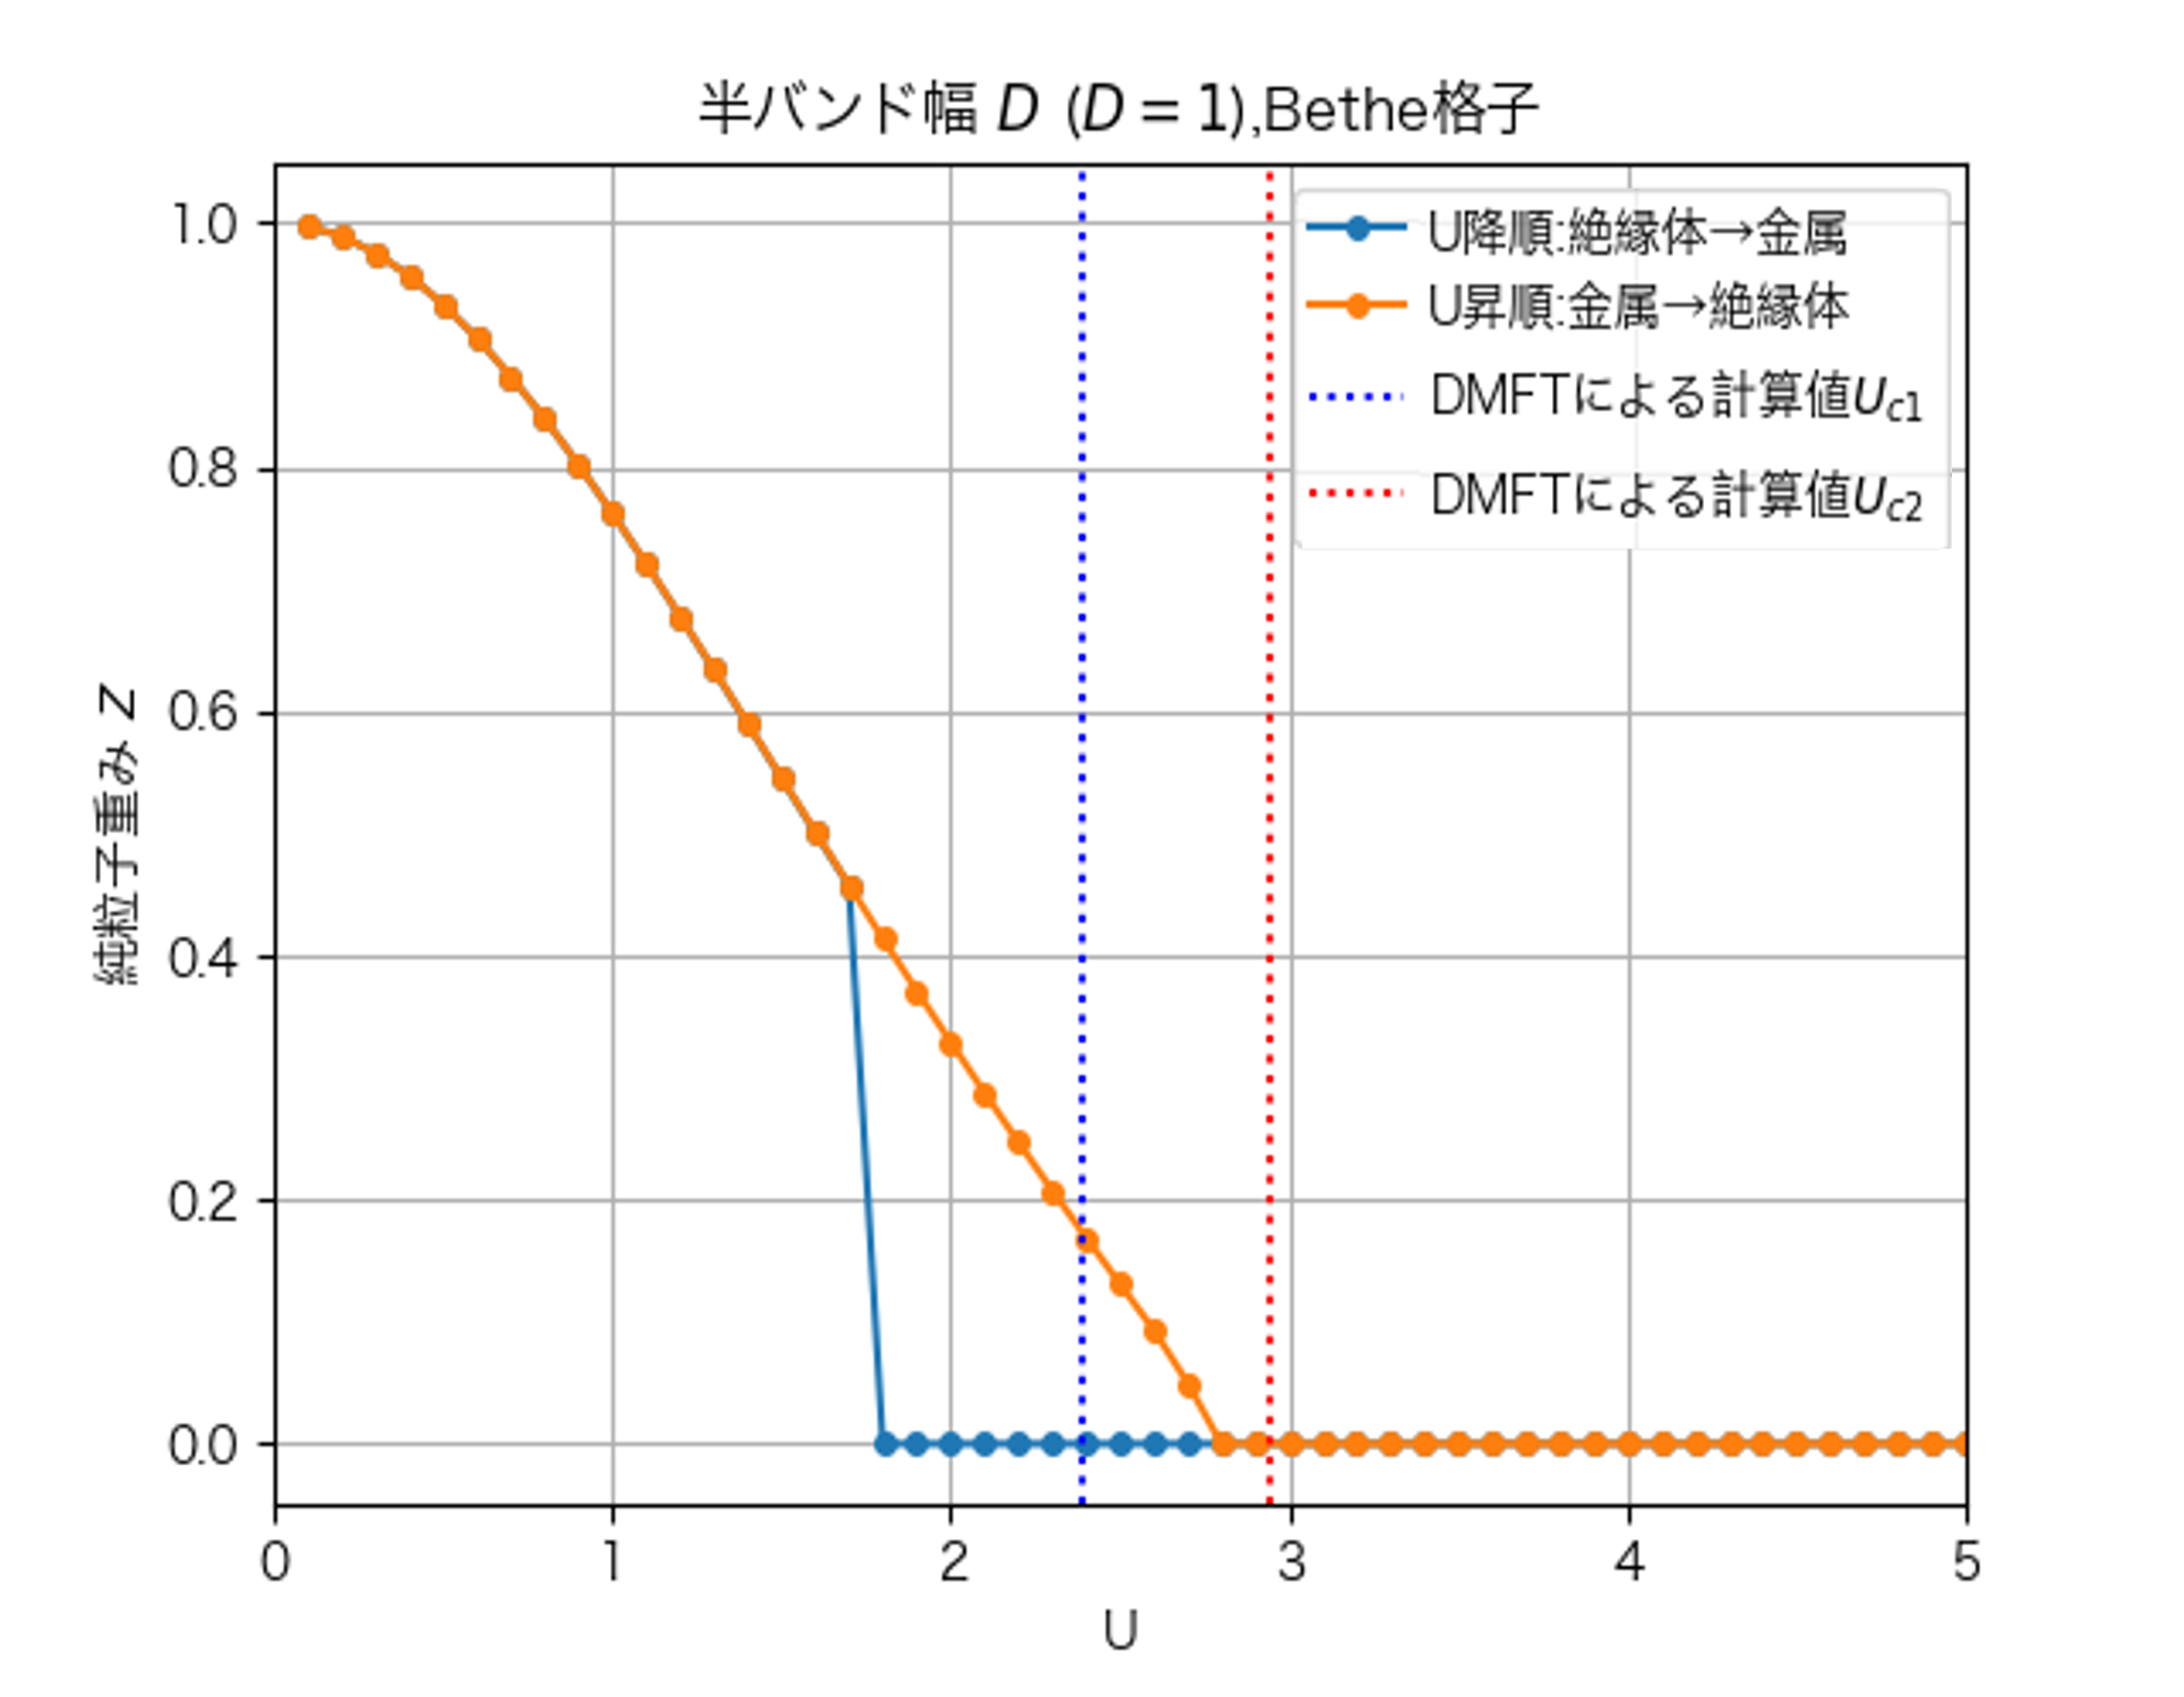
\includegraphics[width=0.9\textwidth]{fig/卒論_Bethe.png}
   %\caption{図の例}
   %\label{fig:sample}
 %\end{figure}

\section{評価指標}

本研究では金属状態とモット絶縁体状態の相転移を判定するための物理的な指標として,準粒子重み$Z$を用いた.

準粒子重み$Z$は電子が相互作用によってどれほど自由電子としての性質を失い,有効質量が増大しているかを表す量である.

$Z > 0$の有限の値を持つ場合は,系がフェルミ液体として振る舞う金属状態であることを意味する.

相互作用の増大に伴って$Z$が減少し,最終的に$Z = 0$となった状態は,電子が各サイトに完全に局在して動けなくなったモット絶縁体状態であることを意味する.

\section{結果}

前章で述べた計算条件に基づき,無限次元Bethe格子および2次元正方格子のそれぞれに対して,クーロン相互作用$U$を変化させた際の準粒子重み$Z$の振る舞いを計算した.

図\ref{fig:result_bethe}にBethe格子における計算結果を示す.

また,図\ref{fig:result_square}に2次元正方格子における計算結果を示す.

% グラフ挿入用のプレースホルダー (ファイル名をご自身の画像に書き換えてください)
 \begin{figure}[H]
     \centering
      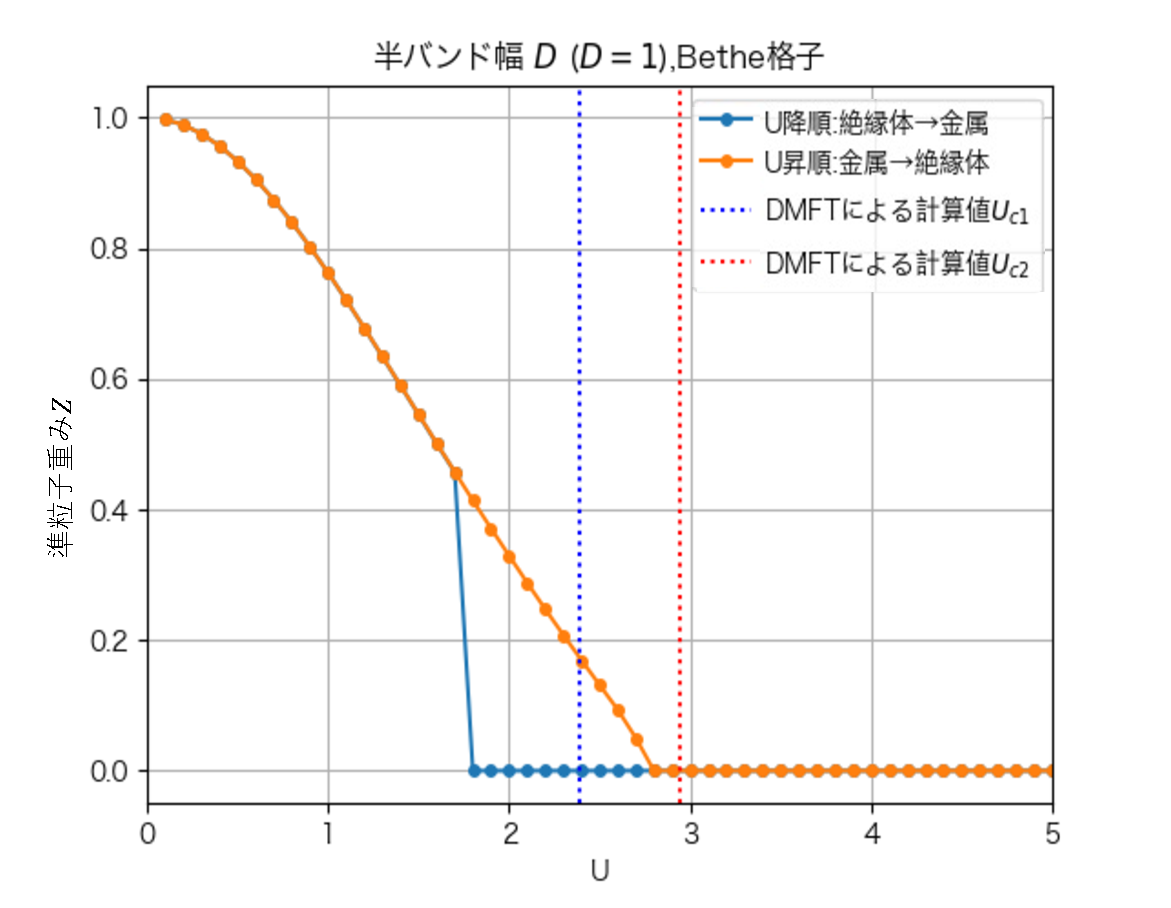
\includegraphics[width=12cm]{fig/卒論_Bethe.pdf}
          \caption{無限次元Bethe格子における準粒子重み$Z$の相互作用$U$依存性.}
    \label{fig:result_bethe}
 \end{figure}

 \begin{figure}[H]
     \centering
      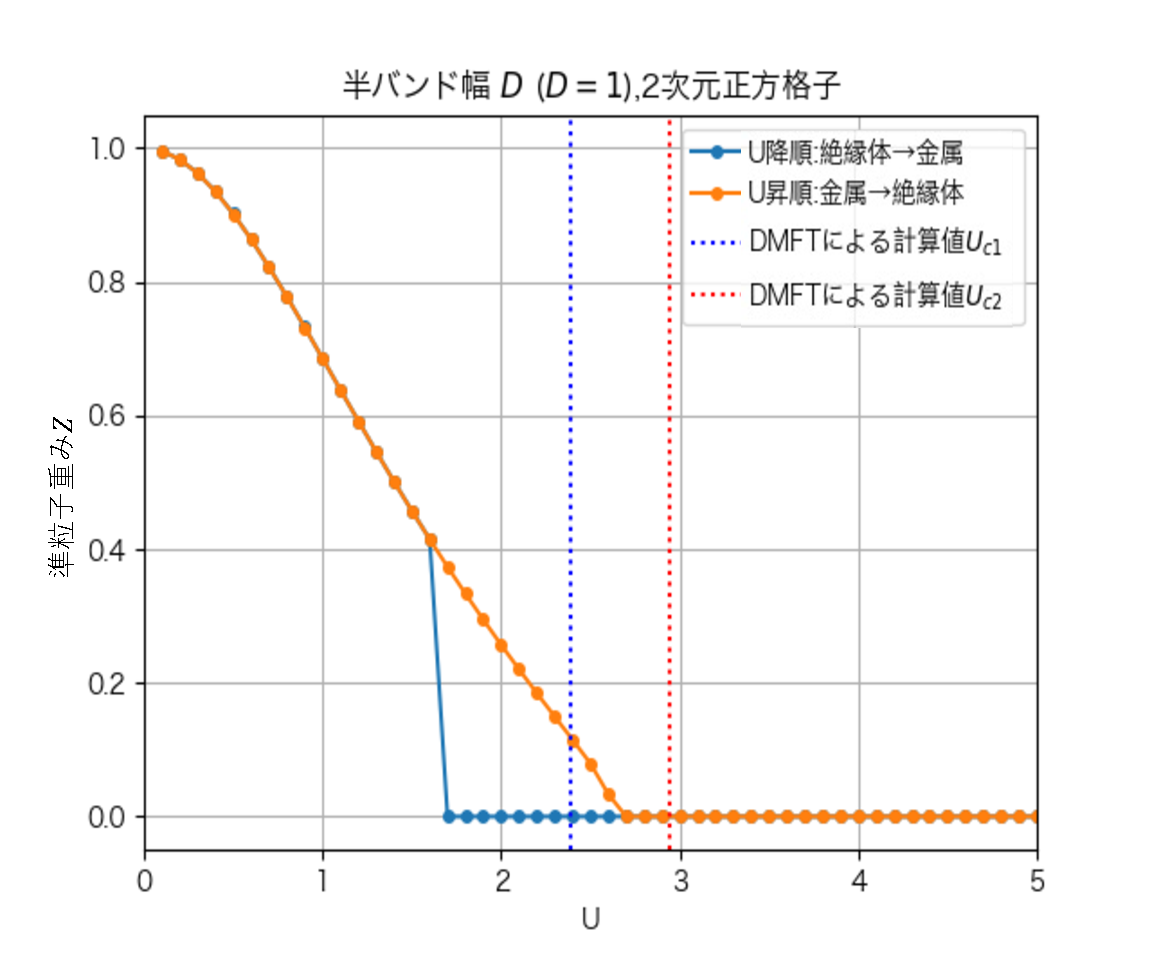
\includegraphics[width=12cm]{fig/卒論_2Dsquare.pdf}
     \caption{2次元正方格子における準粒子重み$Z$の相互作用$U$依存性.}
     \label{fig:result_square}
 \end{figure}

両方の格子モデルにおいて,相互作用$U$が小さい領域では$Z$が1に近い有限の値を取り,金属状態であることが確認できる.

$U$を増加させていくと電子相関の効果によって$Z$は単調に減少し,ある臨界値で不連続に$Z=0$へと落ち込む一次相転移の振る舞いが見られた.

さらに,金属相を初期値とする昇順スイープと,絶縁体相を初期値とする降順スイープで異なる経路をたどるヒステリシスループが明確に観測された.

このヒステリシスの存在は,金属状態の解とモット絶縁体状態の解が共存する領域があることを示している.

\section{考察}

本研究で得られた計算結果を,無限次元において厳密となる動的平均場理論による結果と比較して考察する.

動的平均場理論の計算によると,Bethe格子におけるモット転移の臨界値は,絶縁体解が消失する転移点が$U_{c1} = 2.39$,金属解が消失する転移点が$U_{c2} = 2.94$であると知られている.

図\ref{fig:result_bethe}に示された結果において,降順スイープで$Z$が立ち上がる点と,昇順スイープで$Z$が消失する点は,これらの厳密な臨界値$U_{c1}$および$U_{c2}$と極めて良い一致を見せている.

これは,補助空間を導入して変分空間を拡張したghost Gutzwiller近似が,モット転移の物理を定量的に高い精度で記述できていることを証明している.

また,次元性の影響を考察するため,Bethe格子の結果と2次元正方格子の結果を比較する.

有限次元の格子モデルである2次元正方格子においても,同様のモット転移とヒステリシスループが観測された.

最後に計算コストの観点から本手法の有用性について述べる.

動的平均場理論において連続時間量子モンテカルロ法などの厳密な不純物ソルバーを用いた場合,膨大な計算時間と並列計算リソースが必要となる.

一方,ghost Gutzwiller近似では単一の計算機を用いた極めて短い計算時間で,動的平均場理論に匹敵する高精度な結果を得ることができた.

この圧倒的な計算コストの低さは,本手法が今後より複雑な多軌道系や大規模な格子モデルへ適用可能な強力な手法であることを示唆している.

\chapter{結論}
% 結論
本研究では,強相関電子系におけるモット転移の性質を明らかにするため,ghost Gutzwiller近似を用いた数値計算を実装し,以下の知見を得た.

\begin{itemize}
    \item \textbf{モット転移とヒステリシスの観測}:
    単一バンドハバードモデルにおいて,相互作用パラメータの増大に伴い準粒子重みがゼロとなる金属絶縁体転移を明確に観測した.

    また,昇順・降順スイープを行うことで,一次相転移に特有のヒステリシスループを捉えることに成功した.

    \item \textbf{厳密解との定量的な一致}:
    無限次元Bethe格子における転移点の臨界値は,動的平均場理論による厳密な計算結果と極めて良い一致を示した.

    これにより,少数のゴースト軌道を用いて変分空間を拡張する本手法が,モット転移の物理を高精度に記述できることが証明された.

    \item \textbf{計算コストの劇的な削減と手法の優位性}:
    動的平均場理論に比べて,本手法は無限個の電子の浴の役割をたった2つの空間ゴースト軌道に押し込めることで,不純物問題を劇的に単純化している.

    厳密対角化を用いて一瞬で解くことができるため,極めて低い計算コストで高精度な結果を得られることが確認された.

    \item \textbf{今後の展望}:
    本手法の計算コストの低さと精度の高さを活かし,今後は多軌道系やより複雑な格子構造を持つ現実の物質の解析へ応用することが期待される.
\end{itemize}

%%%%%%%%%%%%%%%%%%%%%%%%%%%%%%　　付録　　%%%%%%%%%%%%%%%%%%%%%%%%%%%%%%
\clearpage
\renewcommand{\appendixname}{付録}
\appendix

%\chapter{付録A}
%% 付録A
ここに付録を書く.



%\chapter{付録B}
%% 付録B
ここに付録を書く.



%%%%%%%%%%%%%%%%%%%%%%%%%%%%%%　　参考文献　　%%%%%%%%%%%%%%%%%%%%%%%%%%%%%%
\clearpage

\addcontentsline{toc}{chapter}{参考文献}
\nocite{*}
\bibliographystyle{apsrev4-2}
\bibliography{main}

%%%%%%%%%%%%%%%%%%%%%%%%%%%%%%　　謝辞　　%%%%%%%%%%%%%%%%%%%%%%%%%%%%%%
\clearpage
\chapter*{謝辞}

% 謝辞\chapter*{謝辞}
%\addcontentsline{toc}{chapter}{謝辞}

本研究を進めるにあたり,多大なるご指導とご鞭撻を賜りました品岡寛准教授に深く感謝申し上げます.

また,日々の研究活動において活発な議論を交わし,有意義な時間を共有していただいた物性理論研究室の皆様に心より御礼申し上げます.

特に,研究室内で定期的にゼミを開いていただき,ghost Gutzwiller近似のレクチャーノートを共に読み進めながら,本研究の基礎から丁寧にご指導いただいた先輩方や同期の皆様には深く感謝いたします.

皆様からの温かいサポートと恵まれた研究環境のおかげで,本論文を無事に完成させることができました.



\end{document}

